\documentclass[a4paper, oneside]{csthesis}

% package to be able to use special characters
\usepackage[latin1]{inputenc}

% Sophisticated math package
\usepackage{amsmath}

% Special symbols
\usepackage{amssymb}

% nicely render theorems and proofs
\usepackage[standard,thmmarks,amsmath]{ntheorem}

\usepackage{graphicx}

% package to format pseudo-code. Check the package documentation.
\usepackage{algorithmic}
\usepackage{algorithm}

% Provides \xspace command that evaluates to a space if the next character in the source is a blank and
% no space if next character is no blank. Useful in command definitions.
\usepackage{xspace}

% Provides a more flexible tabular environment
\usepackage{tabularx}

% Enables the use of the H location specifier for float environments that puts the float exactly where it is located in the source.
\usepackage{float}

% Enables the use of colours
\usepackage{color}

% Enable listings to embed code
\definecolor{lightgray}{gray}{0.95}
\definecolor{darkblue}{rgb}{0,0,.5}

\usepackage{listings}
\usepackage{courier}
\lstset{
         basicstyle=\footnotesize\ttfamily, % Standardschrift
         %numbers=left,               % Ort der Zeilennummern
         numberstyle=\tiny,          % Stil der Zeilennummern
         %stepnumber=2,               % Abstand zwischen den Zeilennummern
         numbersep=5pt,              % Abstand der Nummern zum Text
         tabsize=2,                  % Groesse von Tabs
         extendedchars=true,         %
         breaklines=true,            % Zeilen werden Umgebrochen
         keywordstyle=\color{red},
         frame=b,
 %        keywordstyle=[1]\textbf,    % Stil der Keywords
 %        keywordstyle=[2]\textbf,    %
 %        keywordstyle=[3]\textbf,    %
 %        keywordstyle=[4]\textbf,   \sqrt{\sqrt{}} %
         stringstyle=\color{white}\ttfamily, % Farbe der String
         showspaces=false,           % Leerzeichen anzeigen ?
         showtabs=false,             % Tabs anzeigen ?
         xleftmargin=17pt,
         framexleftmargin=17pt,
         framexrightmargin=5pt,
         framexbottommargin=4pt,
         backgroundcolor=\color{lightgray},
         showstringspaces=false      % Leerzeichen in Strings anzeigen ?
 }
\lstloadlanguages{% Check Dokumentation for further languages ...
         %[Visual]Basic
         %Pascal
         %C
         %C++
         %XML
         %HTML
         Ruby
 }
% \DeclareCaptionFont{blue}{\color{blue}}

  %\captionsetup[lstlisting]{singlelinecheck=false, labelfont={blue}, textfont={blue}}
\usepackage{caption}
\DeclareCaptionFont{white}{\color{white}}
\DeclareCaptionFont{black}{\color{black}}
\DeclareCaptionFormat{listing}{\colorbox[cmyk]{0.43, 0.35, 0.35,0.01}{\parbox{\textwidth}{#1#2#3}}}
\captionsetup[lstlisting]{format=listing,labelfont=white,textfont=white, singlelinecheck=false, margin=0pt, font={bf,footnotesize}}
\captionsetup{format=listing,labelfont=white,textfont=white, singlelinecheck=false, margin=0pt, font={bf,footnotesize}}


\usepackage{subcaption}
\DeclareCaptionFormat{subformat}{\colorbox[cmyk]{0,0,0,0}{\parbox{\textwidth}{#1\hspace{5pt} #2#3}}}
\captionsetup[sub]{format=subformat,labelfont=black,textfont=black}


% Enables clickable links in the PDF and additional PDF specific configuration options.
\usepackage[
            colorlinks=true,
            linkcolor=darkblue, urlcolor=darkblue, citecolor=darkblue,
            raiselinks=true,
            bookmarks=true,
            bookmarksopenlevel=1,
            bookmarksopen=true,
            bookmarksnumbered=true,
            hyperindex=true,
            plainpages=false,
            pdfpagelabels=true,
            pdfstartview=FitH,
            pdfstartpage=1,
            pdfpagelayout=OneColumn
            ]{hyperref}


% link to website in footnote automatically
\newcommand\fnurl[2]{%
  \href{#2}{#1}\footnote{\url{#2}}%
}

% Load own command definitions, a few helpful ones are already defined there.

% This alters the numbering of theorems and lemmas.
\theoremsymbol{\ensuremath{\scriptstyle \Diamond}}
\renewtheorem{theorem}{Theorem}[chapter]
\renewtheorem{lemma}[theorem]{Lemma}
\renewtheorem{corollary}[theorem]{Corollary}
\renewtheorem{definition}[theorem]{Definition}

% This creates a two new theorem-like environments
\theoremsymbol{}
\newtheorem{notation}[theorem]{Notation}
\theorembodyfont{}
\newtheorem*{problem}{Problem}

% This changes the comment style of the "algorithmic" pseudocode package
\renewcommand\algorithmiccomment[1]{\hfill \small \(\triangleright\) #1}

% This creates four commands to leave annotations in your document
\newcommand{\TODO}[1]{\noindent {{\color{red}\fbox{\sffamily \bfseries TODO}} \sffamily #1}}
\newcommand{\FIXME}[1]{\noindent {{\color{green}\fbox{\sffamily \bfseries FIXME}} \sffamily #1}}
\newcommand{\CONSIDER}[1]{\noindent {{\color{blue}\fbox{\sffamily \bfseries CONSIDER}} \sffamily #1}}
\newcommand{\RW}[1]{\noindent \color{blue}#1}


% enable dashed lines
\usepackage{etex}
\usepackage{arydshln}

%  put each section on a new page
\usepackage{titlesec}
\newcommand{\sectionbreak}{\clearpage}

% more space in tables
\setlength{\tabcolsep}{10pt}
\renewcommand{\arraystretch}{1.2}

% make a cell span over multiple rows
\usepackage{multirow}
% and to rotate them
\usepackage{rotating}

% add support for checkmark
\usepackage{pifont}% http://ctan.org/pkg/pifont
\newcommand{\cmark}{\ding{51}}%
\newcommand{\xmark}{\ding{55}}%

%%%%%%%%%%%%%%%%%%%%%%%%%%%%%%%%%%%%%%%%%%%%%%%%%%%%%%%%%%%%%%%%%%%%%%%%%%%%%%%%%%%%%%%%%%%%%%%%%
% DOCUMENT METADATA

\thesistype{Master Thesis\\[5pt]CONFIDENTIAL}
\title{Fraud Prevention and Detection\\[5pt] in Mobile Payments}

\author{C\'{e}dric Waldburger}
\email{wcedric@ee.ethz.ch}
\institute{Distributed Computing Group \\[2pt]
Computer Engineering and Networks Laboratory \\[2pt]
ETH Zurich}

% You can put in your own logo here "\includegraphics{...}" or just comment the command
% \logo{}

\supervisors{Christian Decker\\[2pt] Conor Wogan (SumUp)\\[2pt] Prof.\ Dr.\ Roger Wattenhofer}

% You can comment the following two commands if you don't need them
\keywords{Fraud Detection, Signature Verification, Mobile Payments, Mobile Applications, Dynamic Time Warping, Hidden Markov Models}
% \categories{ACM categories go here.}

\date{\today}

%%%%%%%%%%%%%%%%%%%%%%%%%%%%%%%%%%%%%%%%%%%%%%%%%%%%%%%%%%%%%%%%%%%%%%%%%%%%%%%%%%%%%%%%%%%%%%%%%

\begin{document}

\frontmatter
\maketitle % do not remove this line

\cleardoublepage

\begin{acknowledgements}

  I would like to thank my advisors Prof. Roger Wattenhofer and Christian Decker from the Institute for Distributed Computing at ETH Zurich for their help and support. I also wish to thank Stefan Jeschonnek, Conor Wogan, Matti Biskup and the whole Software Development Team at SumUp for their continuous support.

\end{acknowledgements}


\begin{abstract}
    Mobile payments have seen a lot of traction recently and a set of companies have emerged around the opportunity of payments processed from mobile devices. We've conducted this work in collaboration with a company that allows merchants to process credit card transactions on their smartphone by using a mobile application and a hardware credit card reader that send transactions to the backend (XX).

    The innovative technology has opened up many new beneficial opportunities for both, merchants and clients. It has also opened new opportunities for fraud in the area of credit card transactions. Being historically prone to fraud, the credit card industry is highly regulated. But as existing anti-fraud regulations are specified for the traditional credit card business, the advances in technology call for new anti-fraud measures.

    We identify two  separate but complementary methods against credit card fraud: \textbf{preventive}, in the form of an automatic, in-depth check of all users during the sign-up process against a database of individuals with high risk status, and \textbf{reactive} by providing mechanisms to verify every transaction's signature in real time with the card holder's previous signatures.

    Our work has shown that the optimization of the check during sign-up is able to reduce the number of unnecessary matches by up to 90 percent which results in a reduction of 8 - 16 hours of the manual work done by the operations team each month. At the same time, we were able to make the system more reliable by reducing the number of false positives by about 50 percent.

    We found that the characteristics of a signature captured by finger on a mobile device are much less stable than those of signatures captured with a pen. To account for the resulting false positives, we propose to use a feedback loop to ensure no transactions are lost. We propose a real time signature verification algorithm that fuses the score of a DTW algorithm, an HMM and a score base on global features.

\end{abstract}

\tableofcontents

\mainmatter % do not remove this line


%%%%%%%%%%%%%%%%%%%%%%%%%%%%%%%%%%%%%%%% CHAPTER INTRODUCTION

\chapter{Introduction}

As smartphones become ubiquitous, they're being used in more and more industries and fields. An application that has seen a lot of traction recently is mobile payments. The usage of the smartphone in this field includes the utilization as an electronic wallet, a virtual bank account and as a payment processing terminal to accept credit cards and other payment methods.
This work focuses on an application of the latter.
The density of smartphones per capita and the computational power of current mobile phones have reached a level where it becomes practical to use phones electronic cash registers.
\fnurl{iZettle}{http://www.izettle.com}, \fnurl{Square}{http://www.squareup.com}, \fnurl{SumUp}{http://www.sumup.com} are just some of the companies which make use of this situation and are enabling merchants to receive payments via their smartphone. This thesis was written in collaboration with SumUp, a mobile payment company located in Berlin.

% \cite{Hanmandlu05} \cite{citeulike:3393241} \cite{citeulike:885135} \cite{1030918} \cite{1227706} \cite{Kim:2005:SED:2156512.2156558} \cite{Coetzer:2004:OSV:1289340.1289385} \cite{711942}

Financial businesses have a higher risk of being the target of fraud attacks than businesses in other industries due to the direct financial gain for fraudsters. On mobile devices, it becomes even more important to build automatic processes to protect the system from fraud as the mobile payments are usually a huge amount of small transactions which makes it unfeasible to monitor all transactions manually. While some security measures are imposed by financial authorities, those rules were made for traditional financial institutions. The new mobile, connected environment not only opens up a lot of beneficial opportunities but also more attack vectors for fraudsters. Therefore it is important to not only respect given guidelines but pro-actively develop new ways and adapt existing guidelines to the specifics of the mobile environment to prevent attacks.

We focus our work on two separate, complementary approaches to reduce the fraud risk for a mobile payment company like SumUp.
We implement in-depth checks of new users during the sign-up process, which allows us to reduce the risk of signing up a high risk user. After screening a new user, suspicious applications are flagged for manual inspection of the information that caused the flagging. As this reduced the amount of accounts that have to be checked manually, we were able to reduce the amount of manual work per sign-up substantially.

The second approach focuses on reactive fraud detection and makes use of the most popular method to authorize credit card transactions in mobile payments: by signature.
Authorization of credit card transactions can be done in various ways. They differ in terms of technical complexity and thus cost, speed at which a transaction can be processed and acceptance by card schemes. The most popular card schemes in Europe are MasterCard, VISA, American Express, Diner's Club and others. Widely used are the three following methods:

\begin{itemize}
\item Swipe And Signature (SAS): The card holder swipes his card through a card reader, the information on the magnetic stripe is read and the transaction is confirmed by signature on the mobile device. This approach has the lowest technical complexity of all three but is easier to attack as the data on the magnetic stripe is not encrypted. Main problem: cards can be copied while the card data is read. Widely deployed in the USA due to high acceptance by card schemes.
\item Chip And Signature (CAS): The card holder inserts his card into a card reader and the encrypted information on the card's chip is used to validate the card against the card terminal. The user authorizes the transaction by signing on the smartphone screen. This is currently the most popular method to authorize payments in Europe on mobile devices. The biggest drawback of using CAS to authorize a transaction is that Visa Europe, even though the technical complexity for such readers is much higher, does not consider this method secure enough and therefore requires an extended flow that requires the client to confirm the transaction with a text message. Except from Visa Europe, all other card schemes consider CAS to be sufficiently secure.
\item Chip And Pin (CAP): A card holder inserts the card into a card reader and enters his Personal Identification Number (PIN) into the reader's pin pad to authorize the transaction. Only after the correct PIN has been entered, the phone is able to read  the data required to process the transaction. The main drawback of this authorization method is its high technical complexity, mainly because the reader must be equipped with a pin pad. This incurs higher costs on both, the hardware and software. Although this process allows to authorize transactions with any card scheme in Europe, the high cost make a widespread use in the short term unlikely.
\end{itemize}

Although authorization with CAS is a lengthy process with VISA cards in Europe as each transaction needs to be confirmed via text message, it is currently the best compromise between speed, cost and an almost universal acceptance by card schemes. SumUp provides merchants with SAS or CAS readers based on the merchant's profile. This means that currently, all transactions are authorized by signature. Also with other providers of the same service, authorization by signature remains the predominant way to authorize transactions. It is therefore of paramount importance that the authorization by signature process is as secure as possible which motivates our research.

We propose an automatic signature verification system based on a set of global features, Dynamic Time Warping (DTW) and Hidden Markov Models (HMM) to make the authorization process more accurate. As the signatures, which are captured by finger, tend to have a high variability and unstable characteristics, our system has to account for false positive matches. To account for that, we propose a system involving a feedback loop. With a feedback loop, transactions are still possible even if a card holder's signature could not be matched to previous signatures while allowing the signature verification to be trained for future authorizations.

Going forward, we refer to the preventive part of our work as \emph{fraud prevention} and the reactive part as \emph{fraud detection}. We use the term \emph{fraud protection} for findings that apply to both, fraud prevention and detection.



\section{SumUp - Card Payments for Everyone}
\label{intro-sumup}

Credit cards enjoy a huge popularity among consumers which is illustrated by the number of credit card holders in the United States of America (USA): In 2008 over 176.8 million people owned a credit card with average of 3.5 cards per card holder. About 60 percent of consumers own a rewards credit card and approximately 51 percent of the USA's population owns at least two credit cards \cite{woolsey2010credit}.

While credit cards are also very popular with consumers in Europe, far fewer businesses in Europe allow customers to pay by credit card than in the USA. This is mostly due to the following reasons:
\begin{itemize}
\item A European business initially pays between 200 EUR and 500 EUR for a credit card terminal
\item There is a monthly subscription fee of 20 EUR to 50 EUR
\item A percentage of each transaction goes to the credit card company. Usually, merchants pay between 2.75 and 5 percent to the card payment terminal provider. Often, a minimal fee is charged for small transactions.
\end{itemize}

It is likely that these costs are higher due to more extensive regulations which require more operational effort. Also, the CAS and CAP devices are more complex than SAS devices and the hardware costs therefore higher in Europe. The simplified mechanics behind a credit card transaction are shown in Figure \ref{fig:credit-card-flow}.

\begin{figure}[tb]
    \begin{center}
        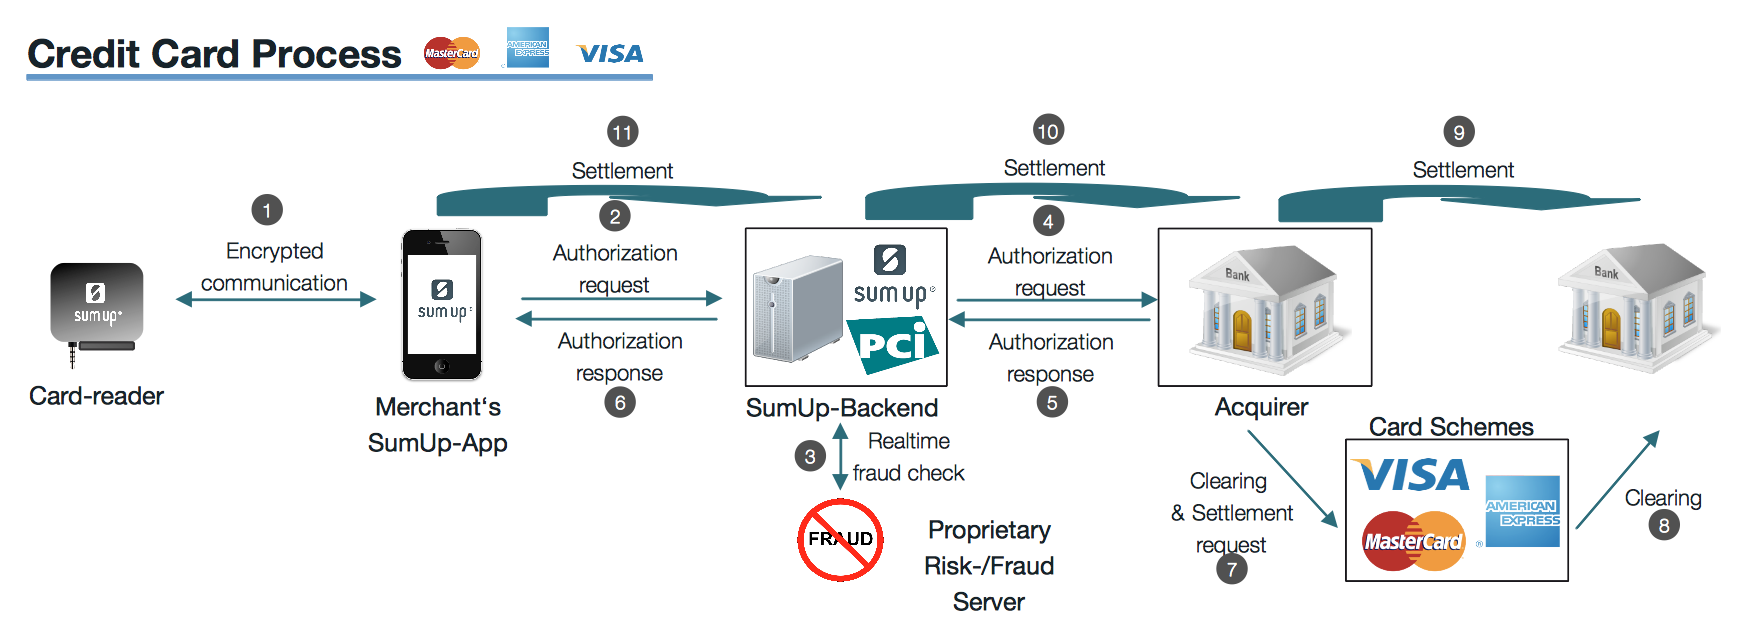
\includegraphics[width=\textwidth]{figures/credit-card-flow.png}
    \end{center}
    \caption{The simplified flow of a single credit card transaction starting with the SumUp CAS credit card reader}
    \label{fig:credit-card-flow}
\end{figure}

SumUp's goal is to lower the barrier for merchants to accept credit card payments by providing a professional yet inexpensive solution for anyone to accept card payments. The company was founded in the fall of 2011 and has enjoyed a rapid growth since.
Today, SumUp's services are used by thousands of merchants in more than ten European countries.
The business has been successful because it removed two out of three of the previously mentioned obstacles to a more widespread adoption: anyone who signs up with SumUp receives a free card reader for use with a smartphone and there is no monthly subscription fee. As the merchant already owns the expensive hardware in form of a smartphone and most people already pay for a data subscription, the cost on both ends is reduced substantially. This way, SumUp is able to finance itself through the 2.75 percent transaction fee. At its core, it competes with traditional credit card terminal providers who require their clients to pay a monthly fee for their terminal and the expensive initial charge for the device.

Instead of building and selling expensive hardware, the only hardware required --- the card reader --- is shipped at no charge and the software is distributed for free via the Apple AppStore and Google Play Store.
Payment through SumUp gives taxi drivers, market traders and other small stores, who couldn't afford one of the traditional payment terminals, an enormous economic advantage. Card payments can now be processed right on the spot and without an initial financial investment.


Processing a transaction with SumUp is illustrated in five simple steps in Fig \ref{fig:flow-customer}.

\begin{figure}
        \centering
        \begin{subfigure}[b]{0.16\textwidth}
                \centering
                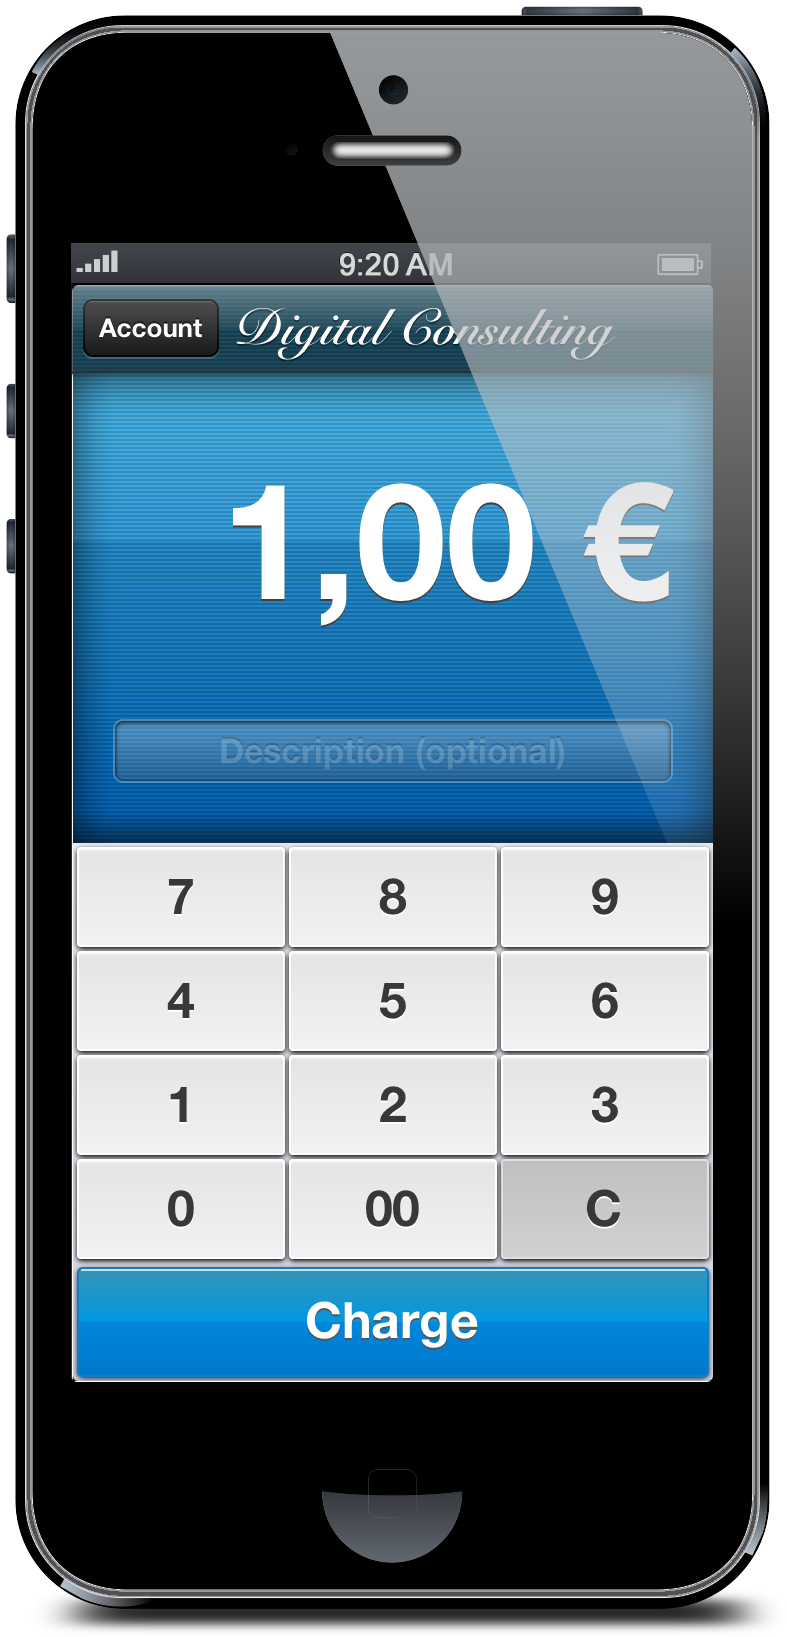
\includegraphics[width=\textwidth]{figures/flow1.png}
                % \caption{Merchant enters amount nto digital cash register}
                \label{fig:flow1}
        \end{subfigure}%
        ~ %add desired spacing between images, e. g. ~, \quad, \qquad etc.
          %(or a blank line to force the subfigure onto a new line)
        \begin{subfigure}[b]{0.16\textwidth}
                \centering
                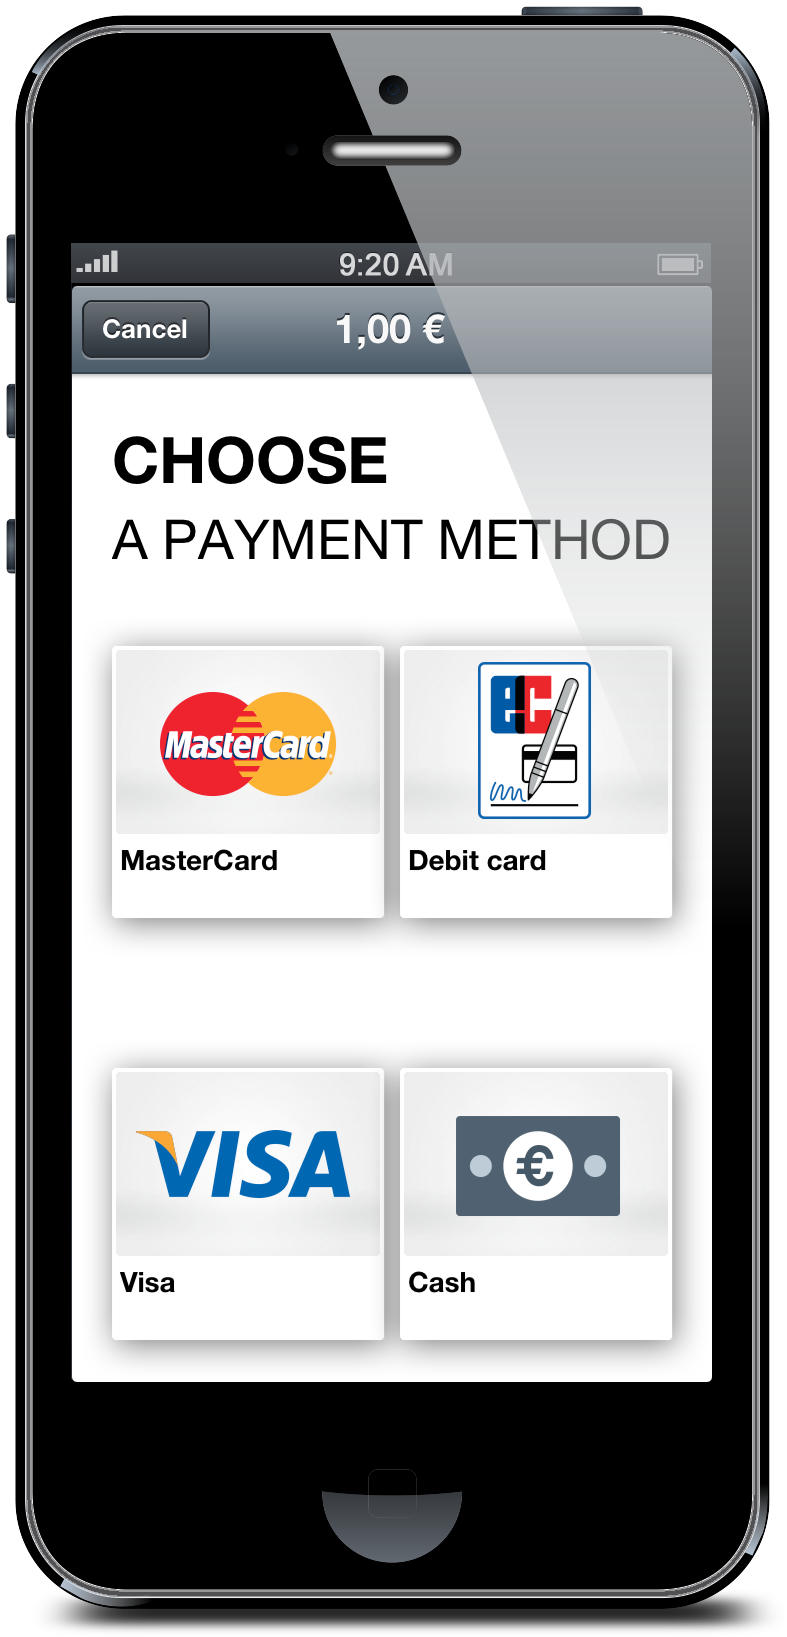
\includegraphics[width=\textwidth]{figures/flow2.png}
                % \caption{Merchant chooes the payment method}
                \label{fig:flow2}
        \end{subfigure}
        \begin{subfigure}[b]{0.16\textwidth}
                \centering
                
\includegraphics[width=\textwidth]{figures/flow3.png}
                % \caption{Once the card reader has been plugged in, the device is ready to read a card}
                \label{fig:flow3}
        \end{subfigure}
        % \begin{subfigure}[b]{0.12\textwidth}
        %         \centering
        %         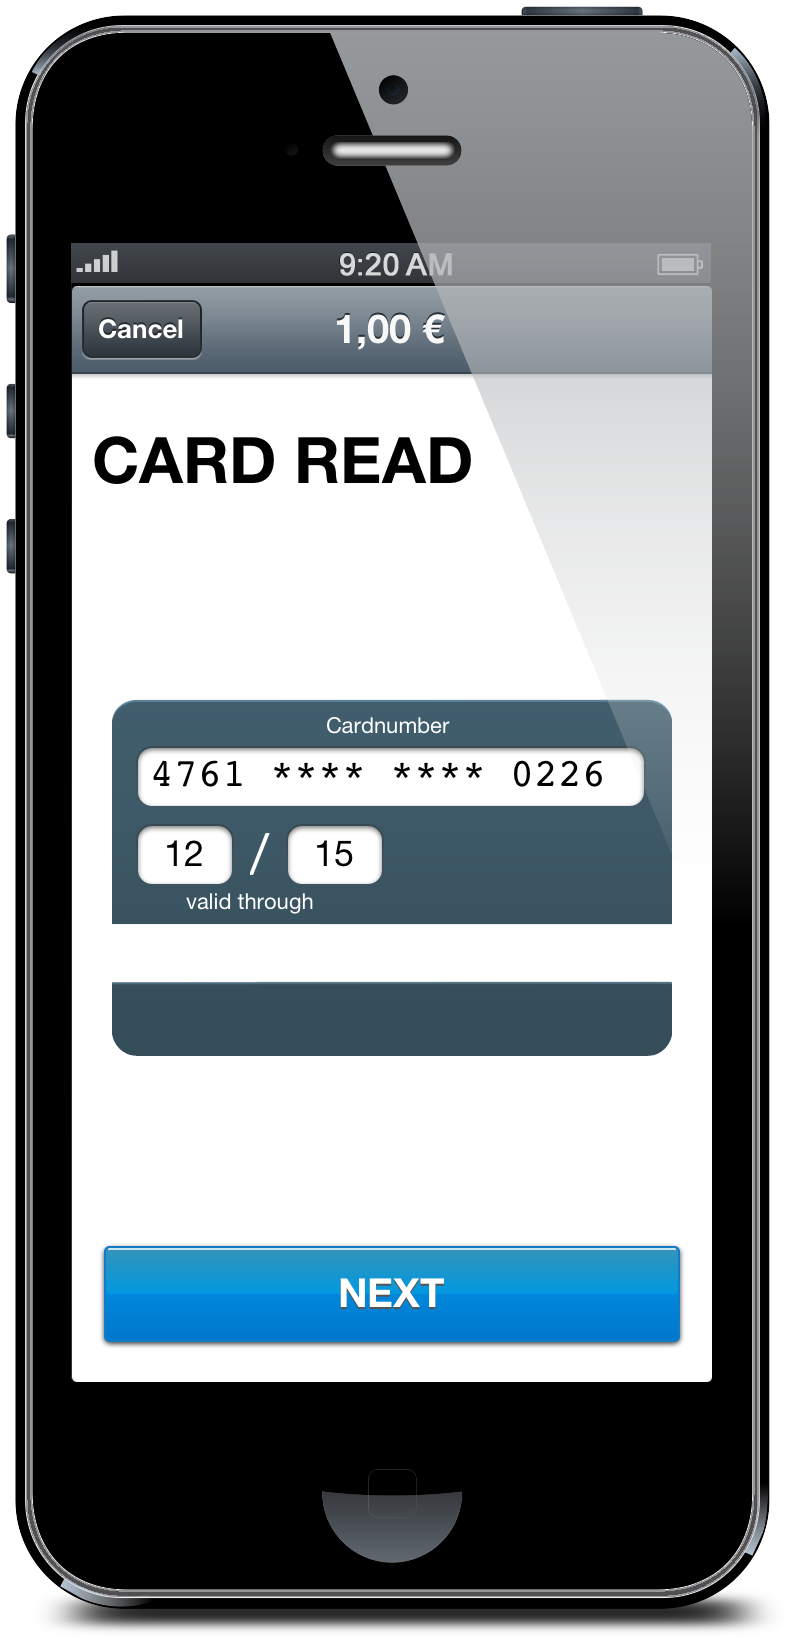
\includegraphics[width=\textwidth]{figures/flow4.png}
        %         % \caption{Card is recognized and shown on the screen}
        %         \label{fig:flow4}
        % \end{subfigure}
        \begin{subfigure}[b]{0.3\textwidth}
                \centering
                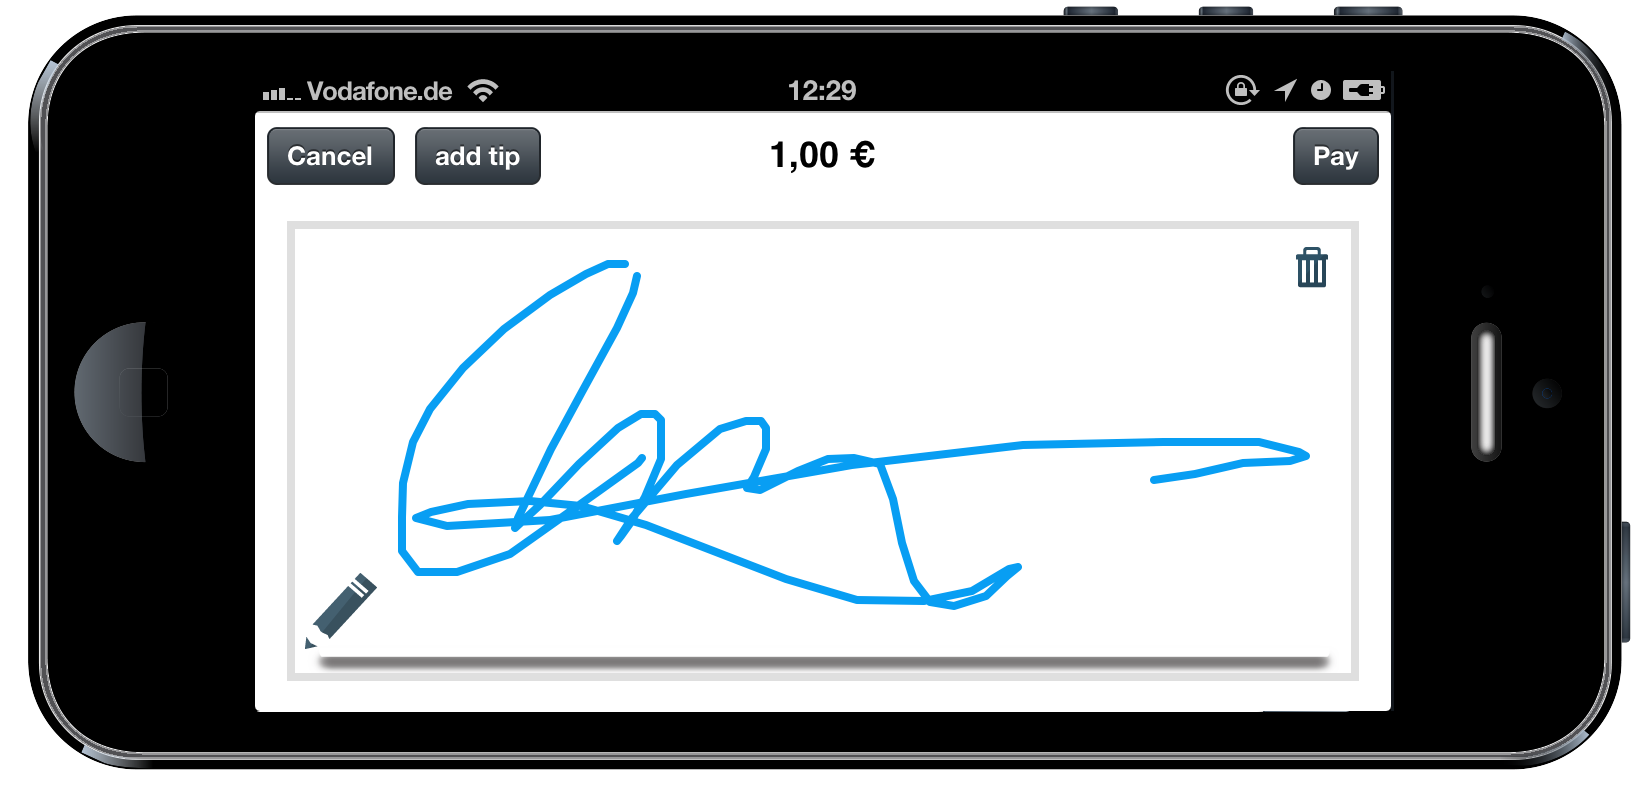
\includegraphics[width=\textwidth]{figures/flow5.png}
                % \caption{Customer signs and thereby confirms transaction}
                \label{fig:flow5}
        \end{subfigure}
        \begin{subfigure}[b]{0.16\textwidth}
                \centering
                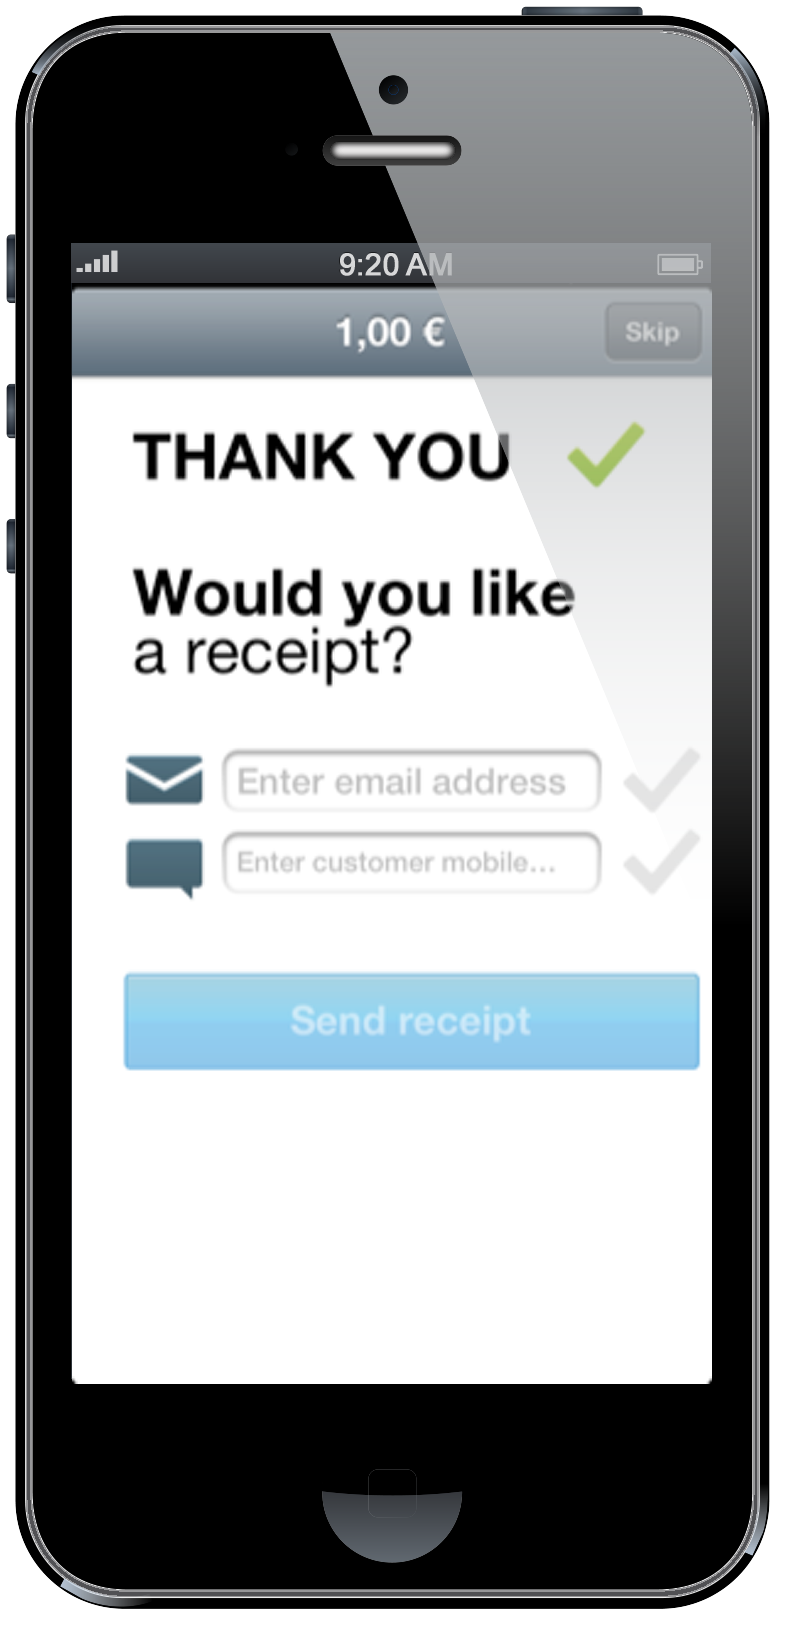
\includegraphics[width=\textwidth]{figures/flow6.png}
                % \caption{Customer can choose to receive a receipt via email or text}
                \label{fig:flow6}
        \end{subfigure}
        \caption{In-App Flow during a Transaction from step 1 to step 5 (from left to right)}\label{fig:flow-customer}
\end{figure}

\begin{enumerate}
\setcounter{enumi}{-1}
    \item Once the merchant has registered a SumUp Account and provided identification documents, he receives a free card reader and can accept payments
    \item The purchase amount can be entered manually into the mobile application or via previously created products
    \item Debit cards and credit cards like Visa and MasterCard are supported and can be chosen by clicking on the respective logo
    \item After reading the card, the mobile application shows a confirmation of the card type and number
    \item The customer confirms the transaction with a signature written onto the screen of the smartphone or tablet
    \item After successful completion, the customer can have the receipt sent to their email account or via text message to their phone
\end{enumerate}


Depending on the authorization method, a number of requests are made to the SumUp servers and from there to other components of the transaction authorization chain, including acquirers, issuing banks and credit card institutions. Internally, a request is sent to SumUp's fraud server which performs a variety of checks and analysis to decide whether the transaction is accepted or declined. There's currently no established third party provider for fraud detection in this area and all rules are custom made by each company. The signature is part of the data that is exchanged with the fraud server and the signature verification process, as described in Chapter \ref{chp:signature-verification}, is an integral part of the  authorization process.

Along with simplicity, quick setup time and low cost, SumUp's advantage over its competitors is that it deducts a relatively low fee per transaction of 2.75\%. From that fee, it also pays the other parties in the value chain. To build a sustainable business model, SumUp will enable customers to also process other types of mobile payments, alongside credit card transactions. The Consumer-To-Business (C2B) credit card transactions will only be one part of all mobile payment transactions. A long term strategy is to implement all payment schemes as listed by the European Payments Council (EPC). Mobile payments may at one point replace all current payment methods for Business-to-Consumer (B2C) transactions as well as Business-to-Business (B2B), Consumer-to-Consumer (C2C) and C2B transactions as listed in Table \ref{fig:mp-applications}. The EPC predicts this will happen due to the availability and convenience of mobile devices paired with the user's perception of having full control over it. This creates an environment of trust and convenience for conducting payments \cite{mpwhitepaper}.


\begin{figure}
        \centering
        \begin{tabular}{c|l}
        \hline
% & 0 & 0 \\ \hline
C2C & Repay a friend \\ \hdashline[0.5pt/3pt]
C2B & Buy Groceries \\ \hdashline[0.5pt/3pt]
B2C & Pay for train to work with company account \\ \hdashline[0.5pt/3pt]
B2B & Pay for Business Lunch \\ \hline
        \end{tabular}
        \caption{Examples of mobile payment applications as listed by the EPC}\label{fig:mp-applications}
\end{figure}


% So funktioniert SumUp:
% Identifizieren und Kartenleser bekommen: Lassen Sie sich mit dem angehängten Formular per Postident identifizieren und wir schicken Ihnen den kostenlosen SumUp Kartenleser zu.
% Starten: Jetzt können Sie Zahlungen von EC- und Kreditkarte empfangen. Nachdem bereits 40% aller Zahlungen mit Karte getätigt werden, verpassen auch Sie nun kein Geschäft mehr! Ob im heimischen Betrieb oder mobil, kein Spontankauf wird mangels Bargeld ausfallen.
% Geld empfangen: Auszahlungen auf Ihr Konto erfolgen jeden Tag, sobald Sie eine Schwelle von nur 20€ Umsatz erreicht haben.
% Kosten: SumUp berechnet eine Gebühr von 2,75% pro Kartenzahlung. Ohne Vertragslaufzeit, ohne Mindestgebühr, ohne Einrichtungsgebühr, ohne monatliche Kosten.


\section{Fraud}

Fraud, as defined by Phua et al. ~\cite{5522816}, refers to the abuse of a profit organization's system without necessarily leading to direct legal consequences. Fraud detection, as part of the overall fraud protection, has become one of the most established applications of data mining.

The large volume of transactions processed each day by SumUp makes a manual verification of each transaction impossible. As such, SumUp has to rely on automated systems to process and validate transactions. At time of this research, there is no established provider of anti-fraud software in this field. However, companies like \fnurl{Sift Science,}{http://siftscience.com} a company which specializes in providing a fraud control service as a third party, has recently raised more than four million USD from leading venture capital firms.

At the time of this work, SumUp does its own internal research to implement, train and tweak its own fraud rules. An internal assessment has shown that the four most popular fraud scenarios are:

% As credit cards are historically a very unsafe payment method, special attention has to be paid when dealing with credit card information and processing credit card transactions.
% A fact that is reflected by looking at how many papers were written about fraud detection in which area. As shown in Figure \ref{fig:fraud-literature-count}.

\begin{itemize}
    \item Money laundry
    \item Copied or stolen cards
    % \item Impersonators transferring money under someone else's name
    % \item Illegal money being transferred through SumUp's system
\end{itemize}

Our fraud prevention mechanisms focus on preventing money laundry while our fraud detection measurements will help to identify a card holder by signature and thereby make it hard for fraudsters to use stolen cards. After a card has been used a certain amount of times, the goal is to  build a reliable signature model to verify it's the same person signing the next time the card is used.

Not only are physical cards at risk to be stolen, also the digital copy of the credit card data needs to be protected. This is one of the reasons SumUp only saves encrypted card information and is obliged to do so according to the Payment Card Industry Data Security Standard (PCI DSS) and in an environment defined by the standard. The standard defines a set of rules to reach these control objectives:
\begin{itemize}
\item Build and maintain a secure network
\item Protect card holder data
\item Maintain a vulnerability management program
\item Implement strong access control measures
\item Regularily monitor and test networks
\item Maintain an information security policy
\end{itemize}

This has an impact on our work as the regulations connected to  protecting card holder data only allow storing card numbers and not names of card holders. The goal of this requirement is that even if someone would gain access to SumUp's database, it would not be possible to retrieve all information needed to process a transaction. This however, bears one disadvantage: we cannot collude information of multiple cards used by a single customer and can therefore only build a signature model based on the signatures we collect per card, not per customer. As the majority of all US card holders holds at least two credit cards \cite{woolsey2010credit}, being able to merge the signature databases from different cards of one card holder, could significantly increase the accuracy of the signature model.

It is impossible to be absolutely certain about the legitimacy of a transaction. In reality, the goal must be to filter out possible evidences of fraud from the available data using cost-effective algorithms in real time.



% \begin{figure}[tb]
%     \begin{center}
%         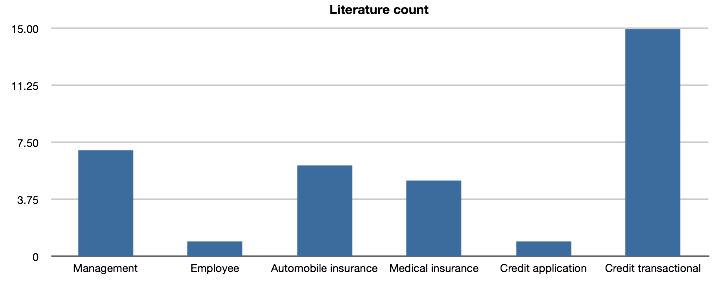
\includegraphics[width=\textwidth]{figures/fraud-literature-count}
%     \end{center}
%     \caption{Number of research papers published on different fraud areas}
%     \label{fig:fraud-literature-count}
% \end{figure}





\section{Signature Verification}

Most previous work on signature detection has been done with signatures captured with a pen on paper or on a digital tablet. When a signature is captured on paper, it was afterwards digitalized using a scanner. The dynamic characteristics of a signature are lost in that process and the algorithms that can be applied to the signature information are very different. Therefore it is common to divide signature verification into two methods:

\begin{itemize}
\item \textbf{Offline signature verification} performs recognition algorithms based on static features of a signature, mainly shape and length.
\item \textbf{Online signature verification} performs algorithms on the dynamic features of a signature. These analyze the speed, the acceleration, the angular acceleration, the pressure and many other local properties of a signature.
\end{itemize}

Since digital tablets, touchscreens interfaces and smartphones became affordable and widely deployed, it became feasible to capture dynamic features of a signature. In Chapter \ref{chp:signature-verification} we look at the common techniques in both areas, offline and online, to verify signatures.

The high accuracy and resolution of current digitizing tablets and smartphone screens enables to capture signature data in high resolution and precision on relatively cheap devices.
Traditionally, digital signatures were captured on a digital tablet with a pen. However, signatures captured by SumUp are collected on a variety of mobile devices and have fundamentally different characteristics than signatures captured on digital tablets. The main reasons for these differences are:

\begin{itemize}
    \item The signatures are captured by finger instead of a pen which is not how people are accustomed to sign. This leads to higher variability and less stable signature models.
    \item Most smartphones don't have a fixed sampling rate but an event-based sampling. Whereas the sampling rate on digital tablets is constant, the rate in signatures captured on smartphones can vary a lot within one signature.
    \item The signatures are captured on a lot of different devices with different screen sizes, resolutions, sensor densities and other device specific characteristics.
\end{itemize}

We have to verify signatures in real time to give instant feedback whether or not a transaction will be authorized. This limits not only the number of algorithms we can use in parallel but also the complexity of our models and our dataset.
We discuss our strategies to overcome the listed difficulties in Chapter \ref{chp:signature-verification}.

% How to approach that without the complicated and expensive chip\&pin device?

% Use signature detection to determine if someone is who he/she claims to be

% Specialties of Mobile Payment Signatures:
% - They don't need to be extracted from a paper background
% - All the info is available (timestamps), digital

% Diverse applications inspired researchers to investigate the feasibility of two distinct categories of automatic signa- ture verification systems: those concerned with the verifica- tion of signature images and those concerned with the veri- fication of signatures that were captured dynamically, using a special pen and digitising tablet. These systems are referred to as offline and online systems, respectively.

% In offline systems, a signature is digitised using a hand- held or flatbed scanner and only the completed writing is stored as an image. These images are referred to as static sig- natures. Offline systems are of interest in scenarios where only hard copies of signatures are available, for example where a large number of documents need to be authenti- cated.
% In the online case, a special pen is used on an electronic surface such as a digitiser combined with a liquid crystal dis- play. Apart from the two-dimensional coordinates of succes- sive points of the writing, pen pressure as well as the angle and direction of the pen are captured dynamically and then stored as a function of time. The stored data is referred to as a dynamic signature and also contains information on pen velocity and acceleration. Online systems are of interest for “point-of-sale” and security applications.

% Since online signatures also contain dynamic informa- tion, they are difficult to forge. It therefore comes as no sur- prise that offline signature verification systems are much less reliable than online systems.


% Various pattern recognition techniques have been ex- ploited to authenticate handwritten signatures (see Section 2). These techniques include template matching techniques [7, 9, 11], minimum distance classifiers [10, 12, 14, 15], neu- ral networks [8, 13, 16], hidden Markov models (HMMs) [17, 18], and structural pattern recognition techniques.
% => p559 coetzer

% Jose L Camino:
% Usually the signature classification methods are divided into two kinds: On-line systems and off- lines systems. The on-line systems parameterize the signature using dynamic characteristics such as how long is the signing process, the inclination of the pencil when signing, the pressure on the pencil on the sheet, the speed of the written line, etc. For that, an electronic pencil is used [4][5][6]. Subsequently a classifier is used to recognize the signature form above parameters. In off-line classification method the signature is written on a sheet and it is scanned. Subsequently, fiom the image scanned, the usual step is parameterize their geometric structure as previous stage to their recognition by a Neural Network based classifier [2,7,8,9].



%%%%%%%%%%%%%%%%%%%%%%%%%%%%%%%%%%%%%%%% CHAPTER FRAUD


\chapter{Fraud Prevention \\PEP \& HRA Detection}

Fraud prevention is applied during the sign-up process of a new user and with the goal to keep high risk users from gaining access to the system.
Any financial institution has a high interest to implement as many anti-fraud mechanisms as possible. With the financial industry being a strictly regulated industry, many precautions are mandatory and described by the governing financial authority. Yet, more mechanisms are added on top of the mandated ones as they provide a competitive advantage.

The financial authority governing SumUp's operations is the United Kingdom (UK) Financial Services Authority (FSA) and the regulatory environment is specified in the Money Laundry Regulations (MLR) from 2007 \cite{website:aml-regulations-2007}. Chapter 2 of the MLR specifies the due diligence that has to be done for every client. As part of the due diligence process, the financial institutions are required to check that the customer does not fall into one of the two following categories:

\begin{itemize}
\item \textbf{Politically Exposed Persons} (PEP) are people who hold a prominent political function. In the United Kingdom this is defined as a national position. Also a PEP's spouse and children are included in this category.

\item \textbf{High Risk Accounts} (HRA) are people who have previously committed a financial crime, been involved in a money-laundering related crime (e.g. dealing with narcotics) or are listed on a government watch list.

\end{itemize}

We will refer to the combination of PEP and HRA as "high risk clients". Any new client needs to be checked against existing lists for both types at sign-up and regularly after the initial sign-up.
If the algorithm returns a positive match with either a PEP or an HRA, a flag is raised in the SumUp Operations Admin Panel (SOAP) and the match has to be confirmed or falsified manually. If the match can be falsified, nothing more needs to be done and the user will continue the sign-up flow. However, if there is a positive PEP or HRA match, different procedures have to be followed.

For an identified PEP match, additional due diligence needs to be done to sign up the client. Additional documents need to be collected that give detailed information about the wealth and assets of said client. After performing the additional due diligence, a client can be signed up but settlements need to be blocked.
A positive match with the HRA list means that the subject cannot be signed up and a Suspicious Act Report (SAR) needs to be filed with the Serious Organized Crime Agency (SOCA). All HRAs are banned from conducting business with any financial institution.

Previous to our work, a test based on only first and last name was already in place but produced a numerous false positive matches. This required a lot of manual work to falsify matches. Our goal was to create a fast, reliable check, requiring as little manual input as possible. Chapter \ref{chp:experiments} lists our results.

In the next section we will present the data of the two databases and their origin before talking about the way we structured the lookup and implementation of our solution.

% two strat agains aml: identify customer, get id \& proof of address
% 2nd mitigating strategy: monitor patterns, activity, ...

% plugged into both: screening at beginning \& end


% sanctions hit => can't trade with him
% report suspicion report

% suspicious act report = sar

% => serious organized crime association

% pep = enhanced customer due diligence
% get more docs, based on wealth and funds

% if we onboard them, we need to block settlements


% Our work is inspired by, amongst others, the potential fi- nancial benefits that the automatic clearing of cheques will have for the banking industry. Despite an increasing num- ber of electronic alternatives to paper cheques, fraud perpe- trated at financial institutions in the United States has be- come a national epidemic. The National Check Fraud Center Report of 2000 [1] states that: “. . . cheque fraud and coun- terfeiting are among the fastest-growing crimes affecting the United States’ financial system, producing estimated annual losses exceeding USD 10 billion with the number continuing to rise at an alarming rate each year.”

% 1: National Check Fraud Center, National Check Fraud Center Report, 2000.

\section{PEP \& HRA Database}


World-Check \cite{website:world-check} is one of the providers of the PEP \& HRA database. It consolidates the list by polling many different lists - including the FBI's Most Wanted LIist, Interpol and others.

The data is supplied in a text file as Comma Separated Values (CSV) and contains information in 26 fields per person. The most important fields are listed in table \ref{tbl:world-check-fields}. Unfortunately, the records are far from complete. A lot of the records are missing some of the important fields like birthday or locations, which makes it hard to falsify a match automatically and sometimes a match falls back on just first and last name correlation. World-Check normalizes the data so that all dates have the same format, city and country names are always spelled the same name and data in one field is always represented the same way.

\begin{table}
    \begin{tabular}{l|p{9cm}}
    \hline
    Field & Value \\ \hline
    uid & unique identifier within the World-Check database\\ \hdashline[0.5pt/3pt]
    last\_name & subject's primarily used last name\\ \hdashline[0.5pt/3pt]
    first\_name & subject's primarily used firs first name \\ \hdashline[0.5pt/3pt]
    aliases & other first/last name combinations that the subject has used\\ \hdashline[0.5pt/3pt]
    alternative\_spelling & alternative spelling of the subject's name\\ \hdashline[0.5pt/3pt]
    category & used to define if subject is a PEP or HRA\\ \hdashline[0.5pt/3pt]
    sub\_category & used to define if subject is a PEP or HRA\\ \hdashline[0.5pt/3pt]
    age & age of the subject \\ \hdashline[0.5pt/3pt]
    dob & the subject's date of birth \\ \hdashline[0.5pt/3pt]
    deceased & information about the subject's death \\ \hdashline[0.5pt/3pt]
    locations & the cities the subject was associated with \\ \hdashline[0.5pt/3pt]
    countries & the countries the subject was associated with \\ \hdashline[0.5pt/3pt]
    further\_information & description and references about the subject \\ \hdashline[0.5pt/3pt]
    external\_sources & information about from which sources the information in the database was extracted \\ \hline

    \end{tabular}

    \caption{Fields of the World-Check database CSV file}
    \label{tbl:world-check-fields}
\end{table}


The full database file is about three gigabytes in size and contains some 1.8 million records of PEPs and HRAs combined. As the database is constantly changing, there's also a daily, weekly and monthly incremental update and delete file, with which the database is kept updated without having to download the full database file every so often.
World-Check is a paid service and the data is retrieved over encrypted HTTPS connection.




\section{Algorithm}

Clearly, parsing three gigabytes of raw data and rebuilding the database each time a new user processes through the sign-up flow is slow and not practical. We therefore chose to parse the needed data into a relational database, allowing us to perform queries within split seconds. The algorithm we used to make the lookup faster, consists of two parts - parsing and lookup.

\textbf{Parsing the data}

The raw data contains only one record per individual but often lists not only one pair of first and last name but many. The additional pairs are retrieved from the aliases and alternative\_spellings fields. For faster lookup, each record from the original CSV file is parsed into multiple records in the database such that there exists one database record for each pair of first and last name combination. We create a record for each permutation of first and last name retrieved from those fields to cover all identities a high risk user might possibly use.
Listing \ref{lst:world-check-parse} shows the algorithm used to create the cross product of all name pairs.

\textbf{Lookup}

To improve the duration of a lookup, the database has an index on first and last name on the PEP/HRA table to speed up the lookup. An index was also generated on the other fields used by the lookup algorithm: Date Of Birth (DOB), deceased, locations (cities) and countries.

To reduce the number of false positives, the lookup uses additional information besides the first and last name to confirm or falsify a match. For each lookup, at least the following information needs to be provided to the algorithm:
\begin{itemize}
\item First and last name
\item Date of birth
\item City
\item Country
\end{itemize}

The algorithm is outlined in Listing \ref{lst:world-check-lookup}. It's output is a set of Know Your Customer (KYC) action and statuses which flag the customer in the system and may restrict him from certain actions, e.g. processing transactions with her account.

\begin{lstlisting}[caption={The Lookup algorithm},label={lst:world-check-lookup}]
def lookup fname, lname, dob, city, country

    # collect all hits on first and last name
    all_hits = verified_hits = []
    all_hits << PEP.find_by_first_name_and_last_name(fname, lname)
    all_hits << HRA.find_by_first_name_and_last_name(fname, lname)

    for record in all_hits

        # skip if peson is already deceased
        next if record["deceased"]

        # parse dob. if the dob in the db is incomplete (eg 1971/02/00)
        # only check the complete parts
        y = record["dob"].year  != 0 ? record["dob"]["year"]  : null
        m = record["dob"].month != 0 ? record["dob"]["month"] : null
        d = record["dob"].day   != 0 ? record["dob"]["day"]   : null

        # now skip if one of the values exists but doesn't match
        next if y && y != dob["year"]
        next if m && m != dob["month"]
        next if d && d != dob["day"]

        # at this point, dob matches or wasn't given
        # now, check city
        next unless record["locations"].contains? city

        # and country
        next unless record["countries"].contains? country

        # all checks passed, add this record to the result set

        verified_hits << record

    end

    # now set KYC status for the proven records
    for r in verified_hits
        set_kyc_status r
    end
end
\end{lstlisting}


\section{Implementation \& Architecture}

The PEP \& HAR check was implemented as a \fnurl{Sinatra}{http://www.sinatrarb.com/} Ruby Applicaton, accessible through a REST interface. It fulfills multiple purposes: It parses the initial or incremental database file, it continuously rechecks all users in the database versus the updated database and also answers requests from the sign-up component.

It uses Ruby \fnurl{ActiveRecord (AR)}{http://guides.rubyonrails.org/active_record_querying.html} to connect to a relational database. The Ruby Sinatra Application runs within a \fnurl{CentOS}{http://www.centos.org/} Linux environment and the linux \fnurl{Crontab Tool}{http://unixhelp.ed.ac.uk/CGI/man-cgi?crontab+5/} is used to run the first two tasks in a constant interval:
\begin{itemize}
\item \textbf{daily:} Each day, the incremental update and delete file are downloaded from World-Check to keep the database up to date.
\item \textbf{weekly:} On a weekly base, each user is screened against the updated database and new hits raise a flag in the operations team's panel for further inspection.
\end{itemize}

The third task, answering requests from the sign-up flow is done via a REST interface. Chapter \ref{chp:experiments} goes into greater detail of how the requests are structured. The system topology is shown in Figure \ref{fig:fraud-arch}.

\begin{figure}[tb]
    \begin{center}
        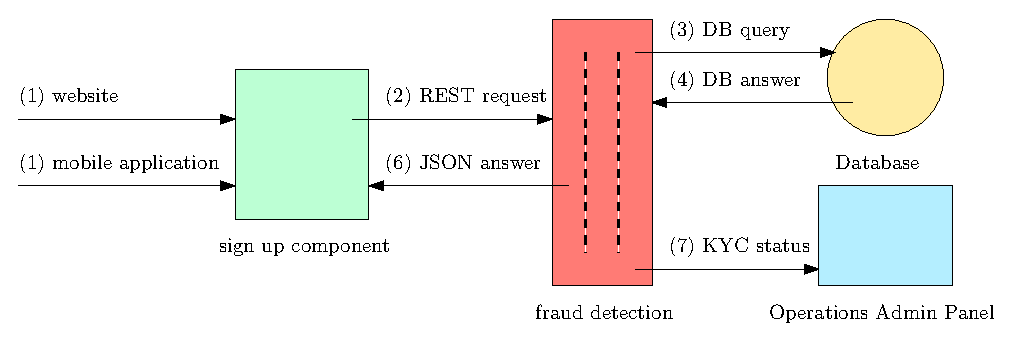
\includegraphics[width=\textwidth]{figures/fraud-arch2.eps}
    \end{center}
    \caption{The simplified architecture and strucutre of a PEP/HRA check request}
    \label{fig:fraud-arch}
\end{figure}

A request is triggered and answered with the following steps:

\begin{enumerate}
\item A new user signs up from one of the mobile apps or the website
\item The sign-up component sends a request for the new user to the fraud detection component
\item The component retrieves the necessary data from the database
\item The database delivers all matches based on first and last name
\item The Lookup algorithm is performed within the fraud detection component
\item The result is returned to the sign-up component with information of whether or not the user can continue the sign-up flow
\item The respective KYC actions and statuses are set in the database.
\end{enumerate}











%%%%%%%%%%%%%%%%%%%%%%%%%%%%%%%%%%%%%%%% CHAPTER Signature Recognition

\chapter{Fraud Detection \\Signature Verification}
\label{chp:signature-verification}

For centuries, being able to authenticate someone based on biometrics, has been important to identify each other, in order to conduct business and verify the authenticity or grant access to resources. In order to guarantee someone's identity, it has always been important to work towards more exact, more reliable means to measure someone's biometric properties and to match recorded properties against known good samples, while at the same time minimizing the chance of an erroneous accept or reject. The characteristic properties of a handwritten signature help to prove a signer's identity. A signature has four legal properties~\cite{Hanmandlu05}:

\begin{itemize}
\item \textbf{Authentication}: Signature verification allows to confirm a signer's identification
\item \textbf{Acceptance}: By signing a document, the writer conveys a willful intent and acceptance of the document's terms and contents
\item \textbf{Integrity}: By signing a document, the signer establishes the integrity of the signed document and that it has not been altered
\item \textbf{Non-repudiation}: The above three factors make it impossible for the signer to deny having signed the document
\end{itemize}

Signature verifications is a particularly important biometric identification process as the signature is a widely accepted method for endorsing financial transactions ~\cite{1227706}.
As the signature is recorded in the SAS and CAS authorization process, it makes sense for SumUp to use this information to improve the security of both authorization methods.

We present existing methods before describing the signature verification methods used in our work and the peculiarities for signature detection in mobile payments.
Traditionally, detection methods can be assigned to either feature- and function-based methods. We describe both approaches in Section \ref{sec:features} and Section \ref{sec:functions}. As a combination of feature- and function-based approaches has been providing better results than the individual techniques \cite{fierrez2005line}, we combine both approaches in our method to verify signatures.

% Theoretically, the problem of handwritten signature verification is a pattern recognition task used to discriminate two classes of original and forgery signatures. A signature verification system must be able to detect forgeries and to reduce rejection of genuine signatures simultaneously.

% Human signature verification (HSV) systems are usually built either on-line or off-line approaches, depending on the kind of data and application involved. On-line systems generally present a better performance than the off-line ones but require the necessary presence of the author during both the acquisition of the reference data and the verification process limiting its use of certain kind of applications.

% A great deal of work has been done in the area of offline sig- nature verification over the past two decades. A recent paper by Guo et al. [11] includes an extensive overview of previous work. Numerous methods and approaches are summarised in a number of survey articles. The state of the art from 1993 to 2000 is discussed in a paper by Plamondon and Srihari [5]. The period from 1989 to 1993 is covered by Leclerc and Pla- mondon [19] and the period before 1989 by Plamondon and Lorette [20]. Another survey was published by Sabourin et al. in 1992 [21]. A review of online signature verification by Gupta and McCabe in 1998 also includes a summary of some earlier work on the offline case [22].
% Earlier work on offline signature verification deals pri- marily with casual and random forgeries. Many researchers therefore found it sufficient to consider only the global fea- tures of a signature.



\section{Global Systems}
\label{sec:features}

Global systems, also called feature-based systems, are characterized by the fact that the feature vector consists of measurements that are based on the signature as a whole. Velocity, acceleration and position are usually looked at either combined or per dimension (usually $x/y$). Popular global features include:

\begin{itemize}
\item Signature length
\item Total time to sign
\item Maximum and average velocity
\item Maximum acceleration
\item Total dots recorded
\item Number of segments
\item Signature Heght (H), Width (W) and W to H-Ratio
\item Number of points with positive $x$/$y$ velocity
\end{itemize}


Global features are derived from the signature as a whole. A lot of research has been done in this area and the features can be simple measurements as those listed or more complicated characteristics obtained through techniques like the discrete Wavelet Transform \cite{ji2005signature}, the Hough Transform \cite{kaewkongka1999off}, horizontal and vertical projections \cite{fang2003off} or smoothness features \cite{fang2001offline}.

% Sequential Forward Feature Selection (SFFS) is one of the best performing methods (TODO: Jain and Zongker, 1997) but many have been proposed. The matching is usually done using statistical classifiers such as Parzen Windows (Martinez-Diaz et al, 2007), majority voting (Lee et al, 1996) Mahalanobis distancis (Galbally et al, 20007) or Guassian Mixture Models (Martinez-Diaz et al, 2007).

% Important features include: \cite{Gueler2008940}





\section{Local Systems}
\label{sec:functions}

% Local features are extracted at stroke and substroke levels and include unballistic motion and tremor information in stroke segments [11], stroke “elements” [9], local shape descriptors [12], and pressure and slant features [13].

% During the past 3 decades, a lot of work has been done on offline and online signature detection algorithms and many techniques exist. Often used local features include:

Function-based systems, also called local systems, are characterized by the fact that the feature vector consists of measurements on individual points or clusters of points.
The most popular methods are Dynamic Time Warping (DTW) and Hidden Markov Models (HMM).

\begin{itemize}
\item Pressure
\item Horizontal ($x$) and vertical ($y$) position
\item Path tangent angle
\item Velocity and acceleration in a particular point
\item Log radius of curvature
\item Pen elevation and pen azimuth (not available in our case as signatures are captured by finger)
\end{itemize}

Typically, a function vector has fewer, or at most as many, dimensions as the signature vector. Matching two signatures means to find an algorithm to match either
\begin{itemize}
\item two feature vectors
\item the vector of the test signature to a reference vector or model
\end{itemize}

Researchers have tried various techniques to match the two feature vectors. Among these techniques are: Dynamic Time Warping \cite{Herbst98onan, citeulike:891512}, Hidden Markov Models \cite{Justino00anoff-line}, directional PDF \cite{drouhard_1996_pr}, stroke extraction \cite{1047809}, synthetic discriminant functions \cite{Wilkinson:91}, granulometric size distributions \cite{615447}, neural classifiers \cite{Bajaj19971}, wavelets\cite{Ramesh1999217}, grid features\cite{Qi19941621} and elastic matching\cite{citeulike:941886} to name a few \cite{PiyushShanker:2007:OSV:1274199.1274423}.

% An overview over previous work was given in a paper by Guo et al.~\cite{Justino20051377}

Before trying one of these advanced techniques, one might try to compare two feature vectors in a simpler manner.
The simplest approach of comparing two feature vectors element by element is to use linear correlation \cite{Plamondon1989107} and calculating the distance between each pair.

This approach has two major drawbacks:
\begin{itemize}
\item It only works if the two vectors have equal length. As signatures always vary a bit, it is rarely the case that two signatures and thus the two feature vectors have equal length.
\item Even if the overall path of the signature is very similar, very often there are parts that are distorted or additional in one of two signatures. Linear correlation isn't able to account for local distortions and would thus create a bad score even if the beginning and end of the signature's path were a perfect match.
\end{itemize}

As both phenomena are very characteristics for signature verification, more advanced techniques are developed. Our work concentrates on Dynamic Time Warping (DTW) and Hidden Markov Models (HMM) as these two techniques have shown most success --- especially when combined --- in previous work \cite{fierrez2005line, citeulike:885135, kashi1998hidden, PiyushShanker:2007:OSV:1274199.1274423,martens1996line}.


\subsection{Dynamic Time Warping}


\begin{figure}
        \centering
        \begin{subfigure}[b]{0.30\textwidth}
                \centering
                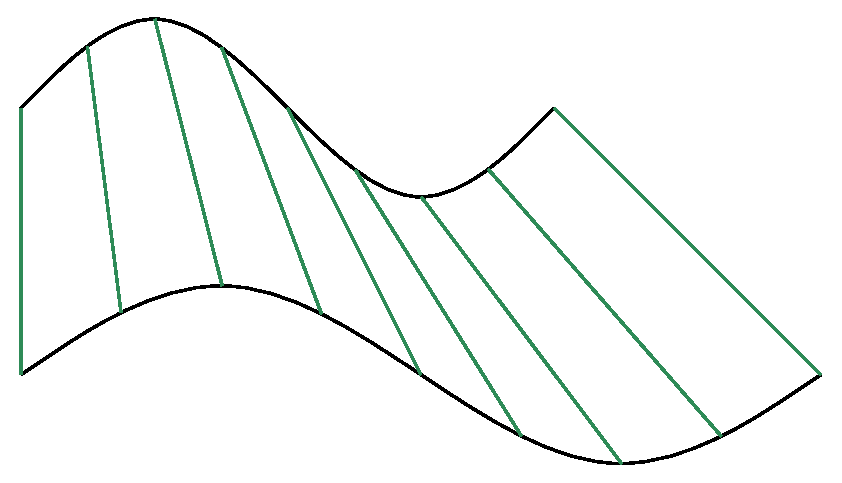
\includegraphics[width=\textwidth]{figures/dtw-stretch.eps}
                % \caption{HMM1}
                \label{fig:hmm1}
        \end{subfigure}%
        \quad
        \begin{subfigure}[b]{0.30\textwidth}
                \centering
                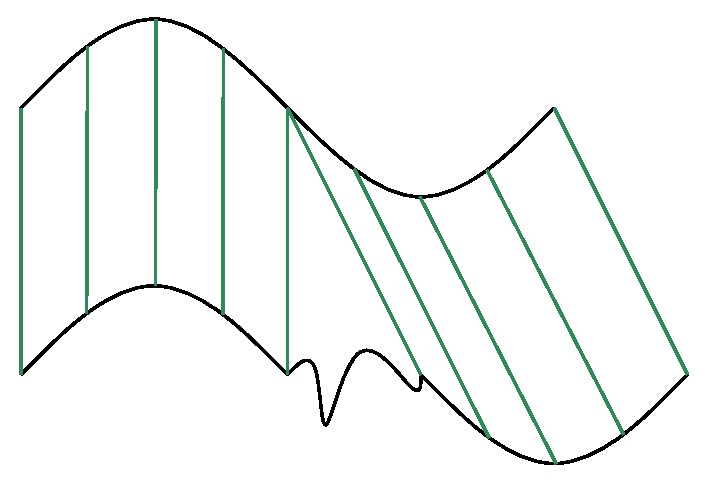
\includegraphics[width=\textwidth]{figures/dtw-distort.eps}
                % \caption{HMM1}
                \label{fig:hmm1}
        \end{subfigure}%

        \caption{Two conceptual drawing of how DTW deals with the two main problems in signature recognition. The time series on the left are stretched but still matched thanks to DTW's ability to account for the scaling of segments or the signature as a whole. The drawing on the right is a representation of how DTW is still able to match two sequences even if one is distorted to a certain degree.}
        \label{fig:dtw-model}
\end{figure}



Dynamic Time Warping (DTW) is a dynamic programming algorithm to measure the similarity between two time series which may vary in time or speed. This has been used for speech recognition and can also be used for signature detection to cope with the non-linear time distortions which one might see in the signals because a signer does not always sign with the same speed. It has shown to be a much more robust distance measure than the Euclidean distance in a simple linear correlation \cite{Keogh:2000:SUD:347090.347153, 1030918, 1227706} due to it's ability to match similar shapes even if they are out of phase in the time axis.

Koegh et al.~\cite{Keogh:2002:EID:1287369.1287405} showed that the mean error rate average over 1000 runs for DTW was an order of magnitude lower than the error rate for the Euclidean distance. However, the DTW algorithm also took approximately 230 times longer to evaluate than the Euclidean distance.
It was first applied to signatures in 1977 by Yasuhara and Oka \cite{yasuhara1977DTW} who concluded that is a very useful approach for online real-time signature verification. Yasuhara and Oka used an adaption of the algorithm that was originally proposed by Sakoe and Chiba \cite{1163055} and tuned the algorithm for the use on signature data.

As Figure \ref{fig:dtw-model} shows, DTW accounts for the two main difficulties when comparing two time series - stretching and distortion. This is of particular importance for our work, as we collect signatures on different devices with different sampling rates and even if a signer signs with the same speed but on two different devices, the two time series have very different length. Additionally, the different devices have different touchscreen sizes and surfaces and it is expected that people will not always complete the signature within the same speed due to different friction forces between the finger and touchscreen and length of the signature path due to a larger or smaller screen.

% \textbf{The concept} behind DTW is a dynamic algorithm that finds the shortest path in a matrix of the distance between each pair of dots. DTW can be used to compare two time series with each other and it is therefore inter


\textbf{Classification} is done by computing the distance DTW distance $dtw[s][t]$ between the model signature $s$ and a test signature $t$ which leads to a DTW score. If the score is below a certain threshold, we will consider the two signatures to match.

\textbf{Training} is done by computing the distance measure $dtw[n][m]$ for all signatures $n, m$ in the set of signatures for a certain user and selecting the signature $s$ with the smallest distance to all other signatures. While there are other techniques, which allow to build and train a signature model based on all the reference signatures, DTW only allows to compare two time series at once. Our strategy is to run new test signatures against the signature that has the lowest average DTW score to all other signature in the training set.


\textbf{Algorithm}: We have two signature vectors $X,Y$ containing data for each point of the signatures:

$$X = x_1, x_2, ... , x_i, ... , x_I$$ $$Y = y_1, y_2, ..., y_j, ..., y_J$$

And the distance between two vectors $i,j$ defined as the 2-norm: $$d(i,j) = ||x_i - y_i||$$

We define a warping path $C$ as $$ C = c_1, c_2, ..., c_k, ..., c_K $$ where each element $c_k$ correspondes to a combination $(x_i, y_i)$.

The algorithm spans an $I \times J$ matrix $G$ between the two signature vectors. The matrix is initialized with $$g_1 = g(1,1) = d(1,1) \cdot w(1)$$ where $g_k$ is the accumulated distance after $k$ steps and $w(k)$ is a weighting function that has to be defined.
In each iteration, $g_k$ is computed as $$g_k = g(i,j) = \min\limits_{c_{k-1}} [g_{k-1}+d(c_k) \cdot w(k)]$$ until both Signatures $X,Y$ have been traversed.

The normalized distance of the two signatures is therefore: $$D(X,Y) = \frac{g_K}{\sum_{k=1}^K w(k)}$$ where $\sum w(k)$ compensates the effect of the length of the sequences.

The definitionen of weighting factors $w_k$ defines the matching between the two signatures. The most common definitionen in literature is one where three types of transitions - deletion, match and instertion - are allowed. The resulting $g_k$ becomes:
$$g_k = g(i,j) = \min \left[\begin{array}{c}g(i,j-1) + d(i,j) \\g(i-1,j-1)+ 2 d(i,j) \\g(i-1,j) + d(i,j)\end{array}\right]$$

The first case corresponds to the case of insertion, the second to a match and the third to an insertion. If in each step, there is a match, the path will go along the matrix' diagonal. Generally, the if the path is close to the diagonal, the signature's are similar and the score thus small.


\begin{figure}
        \centering
        \begin{subfigure}[b]{0.45\textwidth}
                \centering
                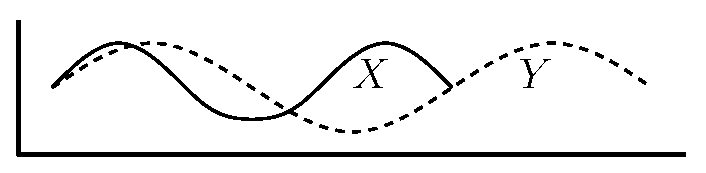
\includegraphics[width=\textwidth]{figures/dtw-graphic1.eps}
                % \caption{HMM1}
                \label{fig:hmm1}
        \end{subfigure}%
        \quad
        \begin{subfigure}[b]{0.45\textwidth}
                \centering
                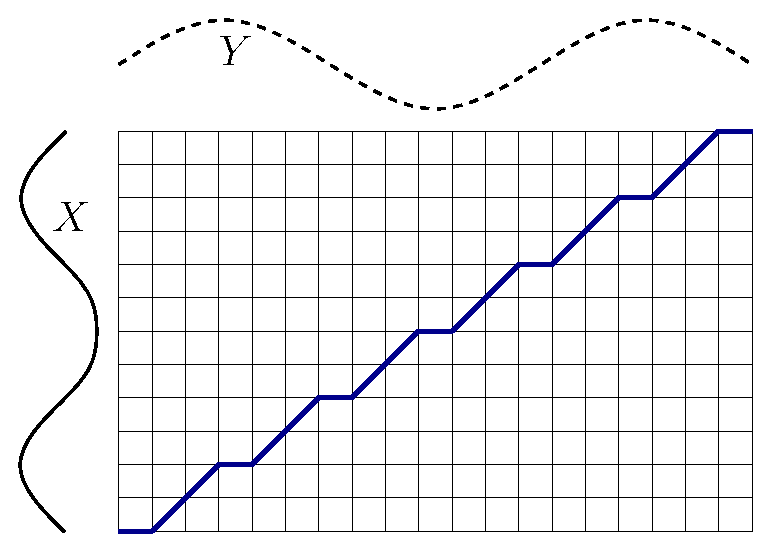
\includegraphics[width=\textwidth]{figures/dtw-graphic2.eps}
                % \caption{HMM1}
                \label{fig:hmm1}
        \end{subfigure}%

        \caption{Two slightly distoreted, strechted time series $X,Y$ can still be matched with the DTW algorithm as the almost perfectly diagonal warping path shows.}
        \label{fig:dtw-matrix}
\end{figure}



Even though the DTW algorithm has been outperformed by more powerful algorithms like HMMs or SVMs in speech detection, it remains very effective in Signature detection as it deals well with small amounts of training data, which is typical for signature verification problems.

In general, DTW is known to have two drawbacks in signature verification:
\begin{itemize}
\item heavy computational load
\item warping of forgeries
\end{itemize}

DTW causes heavy computational load because it does not obey the triangular inequality and thus indexing a set of signatures takes a lot of time. As soon as the pool of signatures for a signer get bigger, the computation costs raise because the test signature has to be compared to each of the signatures in the pool of confirmed signatures. Eamonn Keogh et al.~\cite{Keogh:2002:EID:1287369.1287405} presented a lower bounding method to index all samples without comparing each of them to each other. This is important was we analyze signatures in real time.

The second drawback can be addressed by looking at how straight or bended the warping path is. A straight warping path indicates that a genuine signature is more likely whereas a curvy warping path indicates a forgery. Work on this has been done by Y. Sato et al.~\cite{Sato1982} but made comparison between different signatures more difficult because it introduces another dimension and thus made computation harder and has hence not found wide spread use.

Hao Feng et al.~\cite{Feng:2003:OSV:961320.961331} proposed another extension of the DTW algorithm, called extreme points warping (EPW) which proved to be more adaptive in the field of signature verification than DTW and reduced the computation time by a factor of 11.  Instead of warping the signature as a whole, they only warp so called Extreme Points that are characteristic to a signer's signature and match the curves between those points linearly.



% Dynamic time warping is a classic dynamic programming algorithm that is also used in speech recognition.

% A signature verification system using DTW is reported by Martens and Clae- sen [14]. DTW is a method to measure the similarity between two sequences which may vary in time or speed. This similarity measure can be used to perform signature verification. Comparing two sequences can be done in many different ways such as correlation, integration of the difference of two signals etc. However all these similarity measures cannot cope with non-linear time distortions which we will have in the signature signals. If a user takes a little longer for the first letter of the signature, the similarity measure should not deteriorate more than if the user was taking a little longer on the last letter. The DTW method allows us to compare two signatures while a small time distortion in the beginning of the signature does not accumulatively deteriorate the similarity measure throughout the whole signature.

% page 10-12

% DTW Signature Verification

% Training the DTW signature verification algorithm is performed by calculating the distance measure (dtw[n][m]) for all pairs of signatures in the training set. The signature with the smallest mean distance measure to all the other signatures is selected as the prototypical signature of the given user.
% The DTW matching score of a signature to be verified is equal to the distance measure dtw[n][m] between the prototypical signature found during training and the signature under test.


% ==
% Although the DTW algorithm has been replaced by more powerful ones such as HMMs or SVMs for speech applications, it remains as a highly effective



\subsection{Hidden Markov models}

% Hidden Markov Models (HMM) have been widely used by the speech recognition community (Ra- biner, 1989) as well as in many handwriting recognition applications (Dolfing, 1998). Sev- eral approaches using HMMs for dynamic signature verification have been proposed in the last years (Dolfing et al., 1998; Fierrez et al., 2007; Muramatsu and Matsumoto, 2003; Van et al., 2007; Yang et al., 1995). An HMM represents a double stochastic process, governed by an underlying Markov chain, with a finite number of states and random function set that gen- erate symbols or observations each of which is associated with one state (Yang et al., 1995). Observations are modeled with GMMs in most speech and handwriting recognition applica- tions. GMMs, which can be considered a single-state HMM, have been also successfully used for signature verification (Richiardi and Drygajlo, 2003).

A Hidden Markov Model (HMM) is a stochastic process with an underlying Markov Model.
Unlike with classical Markov Models (MM), the states of a Hidden Markov Model can not directly be observed. Only the symbols emitted from Model's states may be observed. If the signature is interpreted as a succession of observed symbols, then we can, given an HMM, calculate the probability of each path through the states in the model. By training the HMM to match the signatures that are known to be genuine we can thus reconstruct a probability of the user matching.


\begin{figure}[tb]
    \begin{center}
        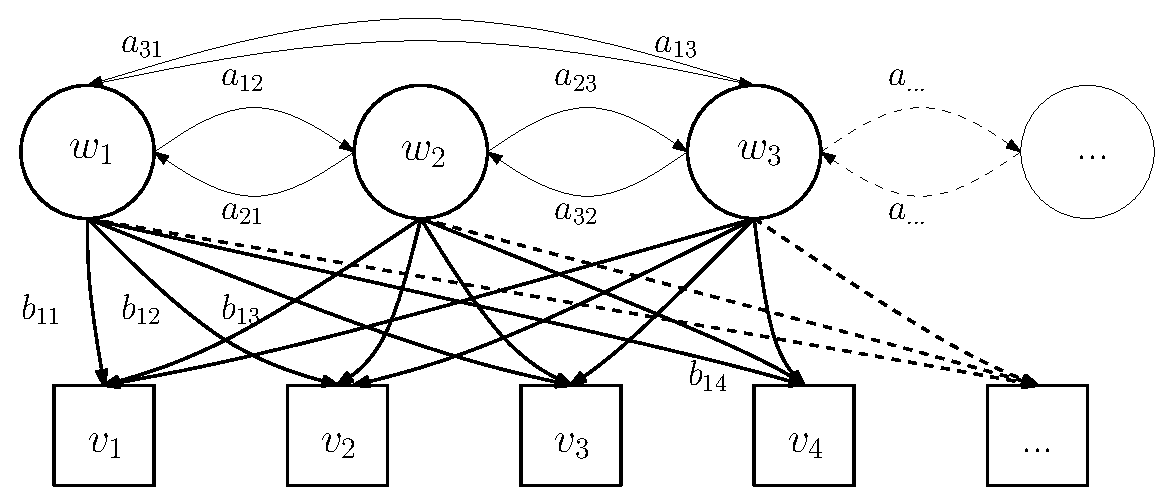
\includegraphics[width=\textwidth]{figures/hmm-general-model.eps}
    \end{center}
    \caption{General representation of an HMM with states $w_1, w_2, w_3, ...$, observations $v_1, v_2, v_3, ...$, the state transition probabilities $a_{ij}$ and the observation emission probabilities $b_{ij}$}
    \label{fig:hmm-general-model}
\end{figure}


An HMM as illustrated in Figure \ref{fig:hmm-general-model} is defined by:

\begin{itemize}
 \item $N$ hidden states $w_1, w_2, ..., w_N$
 \item the alphabet of $M$ of symbols $v_1, v_2, ...$
 \item the $N\times N$ transition matrix $A$, which fulfills
 $$\forall i,\qquad \sum_{j=1}^{N} a_{ij} = 1$$
 and which elements are defined by
 $$a_{ij} \geq 0, \qquad a_{ij} = P(w_j(t+1)|w_i(t)), \qquad 1 \leq i,j \leq N$$

 \item the $N \times M$ emission matrix $B$, which fulfills
 $$\forall i,\qquad \sum_k b_j(k) = 1 $$
 and which elements are defined by
 $$b_j(v(t)) = P(v(t)|w_j(t))$$

 \item the initial distribution $\pi$
\end{itemize}



The underlying Markov Model of an HMM is modelled depending on the application. The most common types are shown in Figure \ref{fig:markov-models}:
\begin{itemize}
\item Left-To-Right HMM (LTR HMM) are characterized by the fact that from each state only the same state or more right state can be reached. Once a state is left, it is never reached again. Depending on the application, no skipping of states (top left), skipping a single step (top right) or skipping an arbitrary number of states may be allowed (mid left). Which states can be reached from which other states is defined by the initial transition matrix. We define our transition matrix in Equation \ref{eq:hmm-transition-matrix} as an LTR model where no states can be skipped.
\item Parallel HMMs have parallel paths, only the states belonging to the same path can be reached once a path is chosen. They have similar properties to LTR Markov Models with the exception that there are multiple paths.
\item Ergodic HMMs are the most generic form of Markov Models where a transition is possible from any state to any other state or the same state. The transition matrix of an ergodic Markov Model has only non-zero elements.
\end{itemize}

In speech and signature recognition, a left-to-right Markov Model has proven to be a good choice. This can be interpreted as that a signer will never go back in his signature, which corresponds to the left-to-right analogy in the time series that corresponds to the signature.

\begin{figure}
        \centering
        \begin{subfigure}[b]{0.35\textwidth}
                \centering
                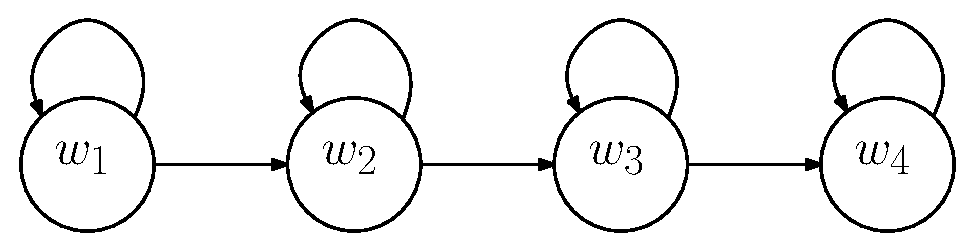
\includegraphics[width=\textwidth]{figures/hmm-ltr1.eps}
                \caption{}
                \label{fig:hmm1}
        \end{subfigure}%
        \quad
        \begin{subfigure}[b]{0.35\textwidth}
                \centering
                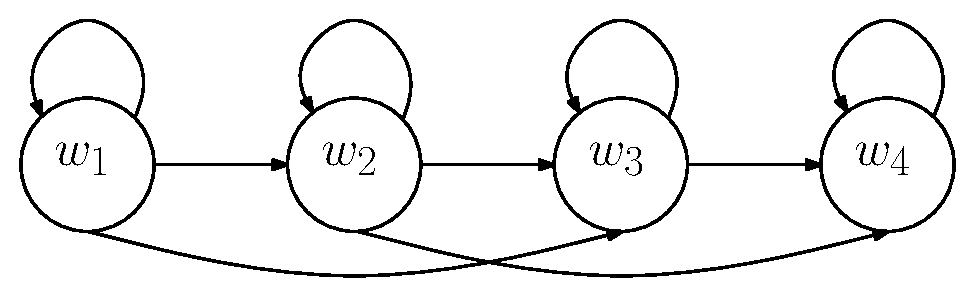
\includegraphics[width=\textwidth]{figures/hmm-ltr2.eps}
                \caption{}
                \label{fig:hmm1}
        \end{subfigure}%

        ~ %add desired spacing between images, e. g. ~, \quad, \qquad etc.
          %(or a blank line to force the subfigure onto a new line)
        \begin{subfigure}[b]{0.35\textwidth}
                \centering
                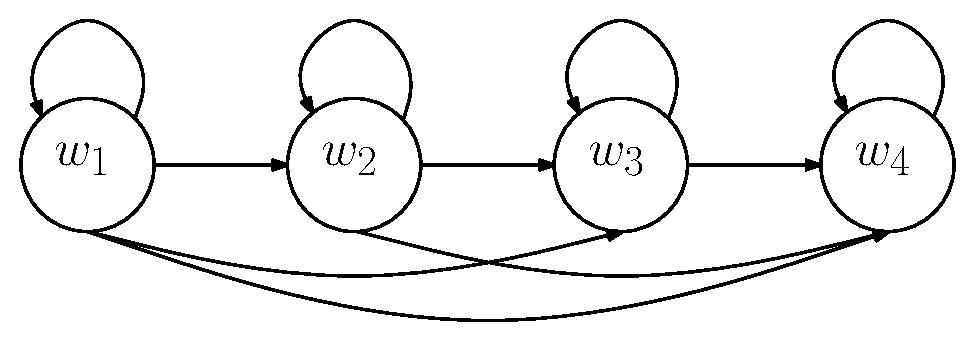
\includegraphics[width=\textwidth]{figures/hmm-ltr3.eps}
                \caption{}
                \label{fig:hmm1}
        \end{subfigure}%
        \quad
        \begin{subfigure}[b]{0.35\textwidth}
                \centering
                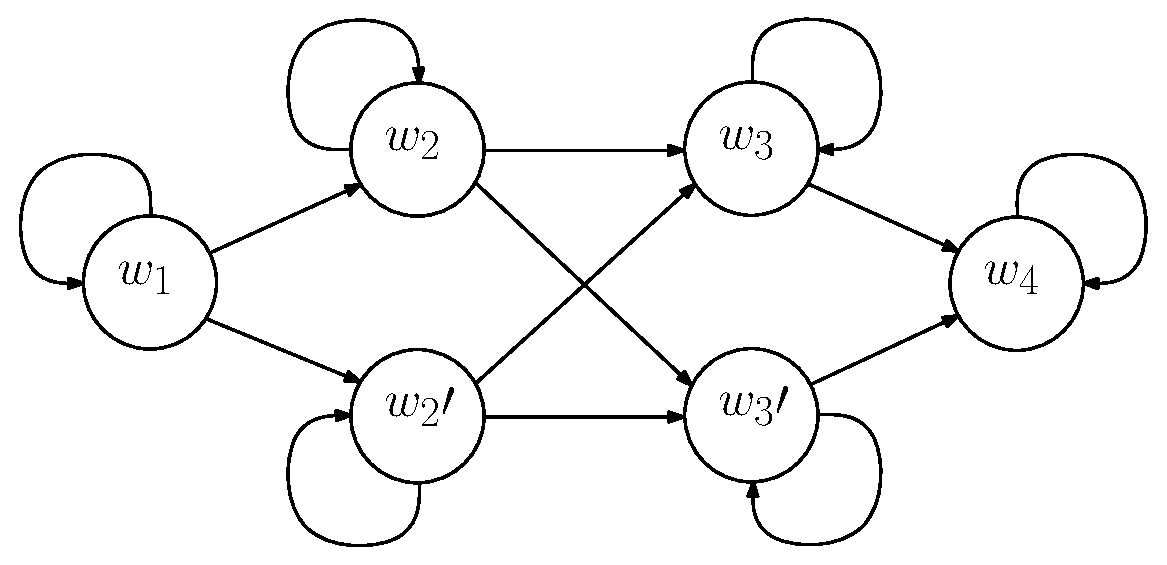
\includegraphics[width=\textwidth]{figures/hmm-ltr5.eps}
                \caption{}
                \label{fig:hmm1}
        \end{subfigure}%

        \begin{subfigure}[b]{0.25\textwidth}
                \centering
                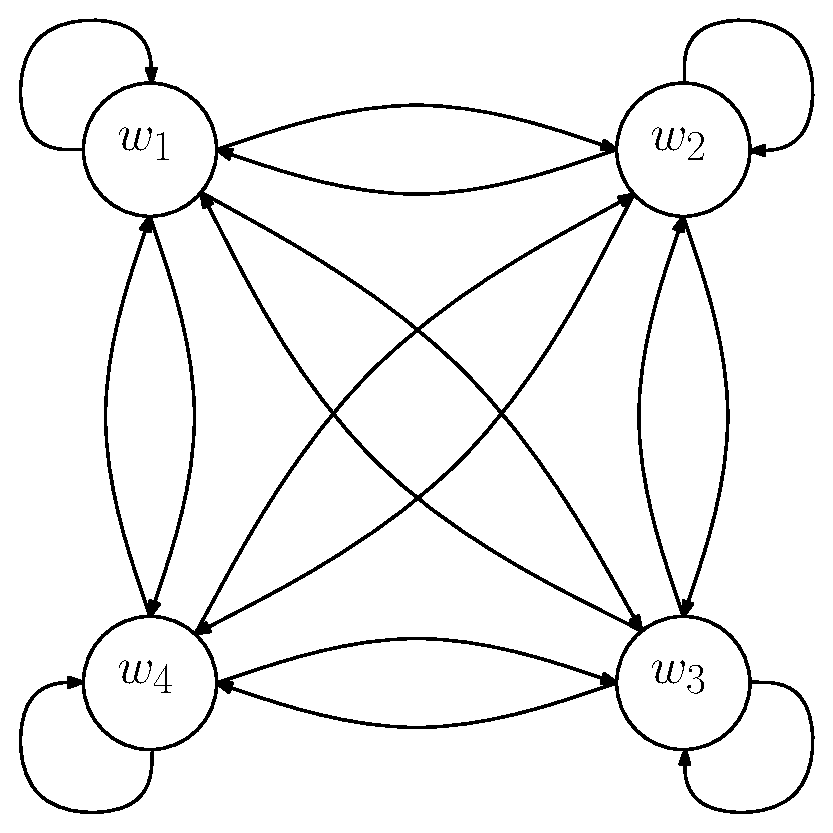
\includegraphics[width=\textwidth]{figures/hmm-ltr4.eps}
                \caption{}
                \label{fig:hmm1}
        \end{subfigure}%



        \caption{Different types of HMMs (from top left to bottom right): LTR HMM where skipping of states is not allowed, LRM with skipping of one step, LRM with allowed skipping, Parallel HMM, Ergodic HMM}\label{fig:markov-models}
\end{figure}



While HMMs with a small set of states and observations perform bad because they are too simple, too many states and observations make the model computational heavy and accuracy is reduced because of overfitting.

The following three problems and their solution are what make HMMs so useful for real world applications:
\begin{enumerate}
\item \textbf{Evaluation}: Given the model parameters and observed data, estimate the optimal sequence of hidden states. This problem is solved by applying the Forward-Backward algorithm to the model.
\item \textbf{Decoding}: Given the model parameters and observed data, calculate the likelihood of the data. This is often solved with the Viterbi algorithm.
\item \textbf{Training}: Given just the observed data, estimate the model parameters. The Baum-Welch algorithm is used to estimate the model parameters.
\end{enumerate}

We are interested in the Evaluation of an observed sequence to match a test signature to one of the signature models and we are interested in the training to train the signature models with the signatures we collect from a card holder. We follow previous authors who used the discretized angle between two points of a signature as the symbols. Based on those symbols, we train our model using the Baum-Welch algorithm. After training signature models, we calculate the likelihood of a signature belonging to a certain card holder by using the Forward-Backward algorithm to compare the signature to this card holder's signature model. A detailed description of all three problems and their solutions is given by Rabiner et al.~\cite{rabiner1989tutorial}.

In our case, we chose to work with an LTR HMM that doesn't allow to skip any states which leads to a transition matrix $A$ of the form:
\begin{equation}
A = \left[\begin{array}{ccccc}a_{11} & a_{12} & 0 & \hdots & 0 \\0 & a_{22} & a_{23} & \cdots & 0 \\\vdots & \vdots & \vdots & \ddots & 0 \\0 & 0 & 0 & a_{(N-1)(N-1)} & a_{(N-1)N} \\0 & 0 & 0 & 0 & a_{NN}\end{array}\right]
\label{eq:hmm-transition-matrix}
\end{equation}


We also chose to work with a LTR HMM that doesn't skip any states and we chose $\pi$ such that the system starts in the first state:
$$\pi = \left[\begin{array}{cccc}1 & 0 & \cdots & 0\end{array}\right]$$


\textbf{The symbols} are calculated as the discretized angle between two points in a signature as illustrated in Figure \ref{fig:hmm-symbol-creation}. We use an alphabet of 4, 8 and 16 symbols in our experiment as described in Section \ref{sec:exp-reactive}.

\begin{figure}[tb]
    \begin{center}
        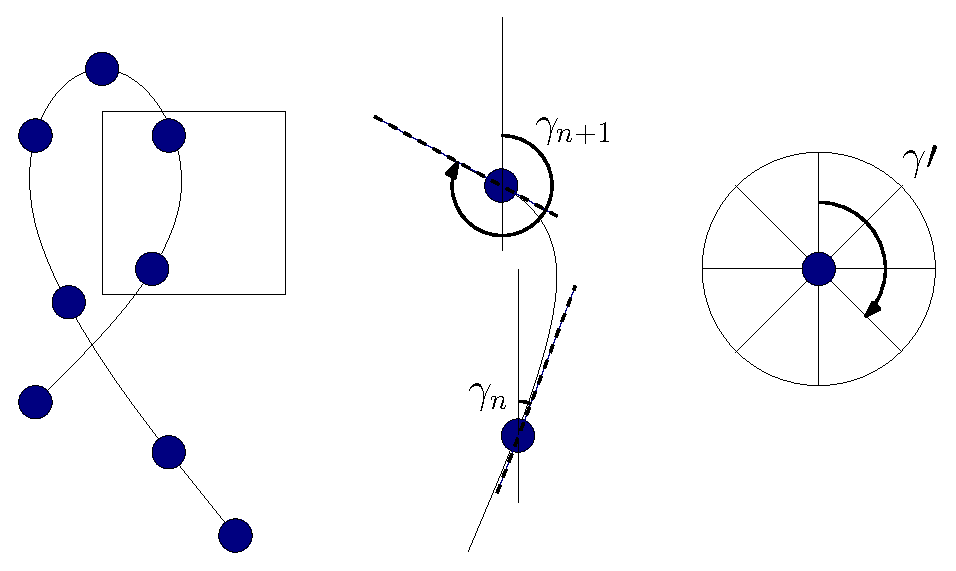
\includegraphics[width=0.6\textwidth]{figures/symbol-creation.eps}
    \end{center}
    \caption{Our symbols are defined as the discretized tangent angle. The left image represents a close up look of a signature and the dots that define it. The drawing in the middle shows a zoomed version of the boxed segment on the right and the tangent angle for the two dots in this area. The right drawing shows the discretized $\gamma\prime$ for an alphabet of 8 symbols.}
    \label{fig:hmm-symbol-creation}
\end{figure}


\textbf{Evaluation: The Forward-Backward algorithm} is a recursive solution. Before looking at the algorithm in detail, we discuss a direct approach to evaluate the probability. A first approach to evaluate which model has produced a certain set of observations might be the following:
\begin{enumerate}
\item For all possible observation sequences, calculate the probability of going from the first to the last state while emitting that sequence
\item These probabilities sum up to the total probability $P(V^T)$
$$P(V^T) = \sum\limits_{r=1}^{r_\text{max}} P(V^T | w_r^T)P(w_r^T)$$
\item For all possible sequences in $w_r^T = w(1), w(2), ..., w(T)$ within $T$ time intervals we get
$$P(V^T) = \sum\limits_{r=1}^{r_\text{max}} \prod\limits_{t=1}^T  P(v(t) | w_(t)) P(w(t)|w(t-1))$$
\end{enumerate}
The problem with this approach is that it is of complexity $\mathcal{O}(N^TT)$ and therefore unfeasible even for small values of N and T. E.g. for $N=5$ States and $T=100$ observations, there are on the order of $100 \cdot 5^100 \approx 10^{72}$ computations.

Clearly, a more efficient way is required. Fortunately, there's The Forward-Backward algorithm is a recursive approach to approximate the solution.

\begin{enumerate}
\item We define the forward-backward variable which is the probability that a model is currently in state $i$ and has already produced the first $t$ elements of $V^T$
$$\alpha_i(t) = \begin{cases} \pi_i b_i(v(0)) & \mbox{if } t = 0 \\ \sum_{j=1}^N \alpha_j(t-1)a_{ij}b_j (v(t))& \mbox{if } t \ne 0 \end{cases}$$

\item For $t=0$ we initialize $a$
$$\alpha_i(0) = \pi_i b_i (v(0))$$

\item We compute $\alpha$ for all states $i$ at all times $t$
\item The total probability that a model $M$ generated the sequence $V^T$ results from the sum of all $\alpha_i(T)$

$$P(V^T|M) = \sum\limits_{i=1}^N \alpha_i(T)$$
\end{enumerate}

This algorithm is only of complexity $\mathcal{O}(N^2T)$ which results in our example to $5^2 \cdot 100 = 2500$ computations. Compared to the $10^72$, a saving of about 69 orders of magnitude --- as long as the number of states is reasonabily low.

In a similar way, we can consider a backward variable $\beta_i(t)$ defined as
$$\beta_i(t) = \begin{cases} 1 & \mbox{if } t = T \\ \sum_{j=1}^N \beta_j(t+1)a_{ij}b_j (v(t+1))& \mbox{if } t \ne T \end{cases}$$
The backward variable $\beta$ defines the probability of the partial observation sequence from $t+1$ to the end. In analogy to $\alpha$, we get the same computational complexity to compute $\beta$.


\textbf{Training: The Baum-Welch algorithm} is used to train signature model. The problem to adjust the model parameters $(A,B, \pi)$ to maximize the probability of the observed sequences is by far the most difficult of the three. There is no analytical way to solve for the model which maximizes the probability. We can, however, find a local maximum with an iterative procedure such as the Baaum-Welch algorithm.
The algorithm's output is the transition matrix $A$ that is most likely to generate the given sequence of observations. The following needs to be known about the model $M$ to start the algorithm:
\begin{itemize}
 \item the number of hidden states $N$
 \item one or more observations sequences $V_1, V_2, ...$
 \item the initial transition Matrix $A$, that defines the HMM's structure
 \item the initial distribution $\pi$
\end{itemize}


In order to get to an iterative solution, we proceed as follows:
\begin{enumerate}
\item We first define the probability of being in state $w_i$ at time $t-1$ and being in state $w_j$ at time $t$ as
$$
\xi_{ij} (t) = P(w_i(t), w_j(t+1)| V^T, M)
\\= \frac{\alpha_i(t)a_{ij}b_j(v(t+1))\beta_j(t+1)}{P(V^T|M)}
$$ $$\\= \frac{\alpha_i(t)a_{ij}b_j(v(t+1))\beta_j(t+1)}{\sum_k = 1^N \sum_l = 1^N \alpha_k(t)a_{kl}b_l(v(t+1))\beta_l(t+1)}
$$

\item By summing over $j$ we get the probability to be in state $w_i$ at time $t$ as
$$\gamma_i(t) = \sum\limits_{j=1}^N \xi_{ij}(t)$$

\item With that, we can calculate the number of transitions from $w_i$ to $w_j$ as
$$\sum\limits_{t=1}^{T-1} \xi_{ij}(t)$$
and the expected number of transitions to any other state as
$$\sum\limits_{t=1}^{T-1} \gamma{i}(t)$$
\item And we get the expected number of times in one state from
$$\sum\limits_{t=1}^T\gamma_i(t)$$
\item With that we can calculate:
\begin{itemize}
\item Expected Frequency (number of times) in state $w_i$ at time $t=0$ $\overline{\pi_i}= \gamma_i(0)$
\item $\overline{a_{ij}} = \frac{\mbox{expected number of transitions from state $w_i$ to state $w_j$}}{\mbox{expected number of transitions from state $w_i$}} = \frac{\sum_{t=1}^{T-1}\xi_{ij}(t)}{\sum_{t=1}^{T-1} \gamma_i(t)}$
\item $\overline{b_j(k)} = \frac{\mbox{expected number of times in state $w_i$ and observing symbol $k$}}{\mbox{expected number of times in state $j$}} = \frac{\sum_{t=1}^T \gamma_i(t)b_i(k)}{\sum_{t=1}^T \gamma_i(t)}$

\end{itemize}

\item Through repeated execution of this algorithm, a local maximum will be found.

\end{enumerate}








% Finding a reliable and robust model structure for dynamic signature verification is not a trivial task. While too simple HMMs may not allow to model properly the user signatures, too complex models may not be able to model future realizations due to overfitting. On the other hand, as simple models have less parameters to be estimated, their estimation may be more robust than for complex models.


% El-Yacoubi [17] uses HMMs and the cross-validation princi- ple for random forgery detection. A grid is superimposed on each signature image, segmenting it into local square cells. From each cell, the pixel density is computed so that each pixel density represents a local feature. Each signature im- age is therefore represented by a sequence of feature vectors, where each feature vector represents the pixel densities asso- ciated with a column of cells. The cross-validation principle involves the use of a subset (validation set) of each writer’s training set for validation purposes. Since this system aims to detect only random forgeries, subsets of other writers’ train- ing sets are used for impostor validation. Two experiments are conducted on two independent data sets, where each data set contains the signatures of 40 and 60 writers, respectively. Both experiments use 20 genuine signatures for training and 10 for validation. Both experiments use the forgeries of the first experiment for impostor validation. Each test signature is analyzed under several resolutions and the majority-vote rule is used to make a decision. AERs of 0.46% and 0.91% are reported for the respective data sets.
% Justino [18] uses a discrete observation HMM to detect random, casual, and skilled forgeries. A grid segmentation scheme is used to extract three features: a pixel density fea- ture, a pixel distribution feature (extended-shadow-code), and an axial slant feature. A cross-validation procedure is used to dynamically define the optimal number of states for each model (writer). Two data sets are used. The first data set contains the signatures of 40 writers with 40 genuine signa- tures per writer. This data set is used to determine the opti- mal codebook size for detecting random forgeries. This op- timised system is then used to detect random, casual, and skilled forgeries in a second data set. The second data set contains the signatures of 60 writers with 40 training signa- tures, 10 genuine test signatures, 10 casual forgeries, and 10 skilled forgeries per writer. An FRR of 2.83% and an FAR of 1.44%, 2.50%, and 22.67% are reported for random, casual, and skilled forgeries, respectively.






% \section{Online Signature Detection}
% % Online signature verification methods are generally categorized to either use global or local features to classify a given signature

% % ==

% % On-line or dynamic systems use captured signature time-functions. These functions are obtained using digitizer tablets or touchscreens (e.g. Tablet-PCs, smart phones, etc.). Tradition- ally, dynamic systems have presented a better performance than off-line systems as more levels of information than the signature static image are available (Plamondon and Lorette, 1989). This is the approach considered in this work, and will be described in the following chapters.

% % Feature Extraction: Two main approaches have been followed in this step: feature- based systems extract global features (e.g. signature duration, number of pen-ups, average velocity) from the signature in order to obtain a holistic feature vector (Lee et al., 1996). On the other hand, function-based systems use the signature time functions (e.g. position, pressure) for verification. Traditionally, function-based approaches have yielded better results than feature-based ones (Fierrez-Aguilar et al., 2005a; Kholmatov and Yanikoglu,
% 2005).


% \subsection{Feature-Based Methods}
% % As the name suggests, feature-based methods use features extracted from the sig- natures to perform the verification task. In general two different types of features are considered: global and local. Global features are related to the signature as a whole, for instance the signature duration or the mean pressure applied. Local features are based on single sample points. Examples for local features are the maximum velocity or the highest curvature.

% % Lee et al. [5].

% % A large number of features useful for signature verification was listed by Fierrez-Aguilar et al. [6].

% % This is why in general a smaller set of more discriminative features is preferred. The issue of feature selection in the signature verification task was extensively studied by Richiardi et al. [7].

% % After having found a suitable feature vector, an arbitrary one-class classifi- cation scheme can be used to perform the classification into valid and invalid signatures. Since there is no negative training data available, the task of classifi- cation is very similar to the task of outlier- or novelty detection. Several methods to perform such a classification are known [8].




% \subsection{Function-Based Methods}

% % Function-based signature verification methods are focused on building a signa- ture model which accurately reflects the temporal behaviour of the signature. Instead of extracting features that are used for verification, the emphasis of the signature model lies in the (timed) sequence of strokes drawn during the signing process. Comparing any signature to the model built during training will lead to a match score which is based on the level of similarity between (timed) sequence of strokes in the model and the signature under test. Function-based methods are reported to deliver better performance than global feature based methods [6]. Two function-based methods are predominant in the literature: Hidden Markov Model based methods and Dynamic Time Warping (DTW) based methods.

% % page 6-8 for sample feature set

% % Function-based methods to perform signature verification compare the tempo- ral behaviour of the recorded signals x(t), y(t), p(t) and a(t). In this work, a dynamic time warping based method is used. The performance of a Hidden Markov Model system might be higher than the DTW system performance but the implementation complexity is much lower for the DTW system.







\section{Challenges in Signature Detection Specific to Mobile Payments}

A lot of work has been done on signature detection on offline and online signatures. However, almost all work on dynamic signatures has been done on signatures that were captured using a pen on a digital tablet. In our case, signatures were captured on a wide range of different devices and with a user's finger instead of a pen.

% Our experiments in chapter X (TODO ref) will show to which extent known techniques are applicable to this type of signature and what future work might need to be done.

\subsection{Signatures are written with Finger}

Our experience shows that people are not used to write their signature with their bare finger and the first few times they sign, their signature differs a lot. However, after just 10-15 times, the signature's shape stabilizes.

This means that it will be a lot harder to detect signatures based on the first few signatures than on later signatures, once a user got used to signing with her finger.
It also means that we should prefer later signatures to earlier ones as in later signatures the signer's signature might have stabilized.


\subsection{Sparse Initial Dataset}

Although SumUp is live in over 10 countries as of today, it is still only used in a relatively small set of locations and we are therefore unlikely to gather a lot of data about a certain user until the concept becomes more often deployed and used.

This means that we have to try and find a solution that works reasonably well with a small amount of initial data per user. The problem persists even after this initial phase as new people will continue to join and always start with an empty set of signatures.


\subsection{Device \& Software Fragmentation}

Unlike signatures captured on a digital tablet, our database of signatures is captured on a variety of devices with different properties. There are various factors that have an influence on the digital representation of the signature:

\begin{itemize}
\item Different Manufacturer: Both, iOS and Android devices use a variety of manufacturers for their handsets and the touch screens used. Recent studies have shown the differences of how signals are captured on different screens (TODO: link reference)
\item Screen Size: the screen diagonal of current smartphones typically ranges between X and X cm, those of tablets typically ranges between X and X cm. A consequence is that the user might not only sign slightly differently but also that the signature will consist of more or less data points and it will take users a longer or shorter amount of time to sign.
\item  ...
\end{itemize}


We will consider these factors when applying our algorithm in Chapter X (TODO)






\section{Feedback Loop}

Due to the mentioned challenges, our systems are likely not to perform as well as the same systems on traditional signatures captured by pen on a digital tablet. We are likely to get results with a higher Equal Error Rate (EER) which would hurt SumUp's business if we declined transactions because of false positive matches.

To eliminate the risk of blocking transactions because of a false positive match, we propose to use a feedback loop along with our signature verification system.

Traditionally, the system would work as shown in Figure TODO


\begin{figure}[tb]
    \begin{center}
        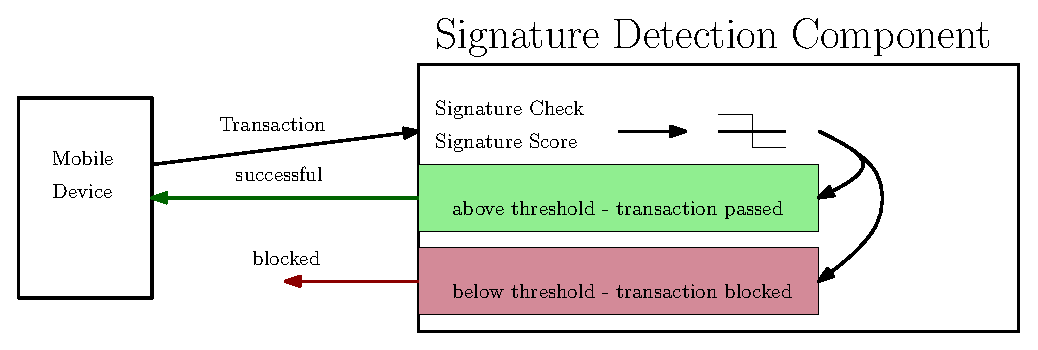
\includegraphics[width=1\textwidth]{figures/fb-loop1.eps}
    \end{center}
    \caption{Simplified illustration of processing a transaction without the feedback loop. When the transaction object is received, the signature is extracted and analyzed. The score is compared with a threshold and if too low, the transaction is blocked. In case of a false positive match, this transaction is lost which we need to avoid.}
    \label{fig:fb-loop1}
\end{figure}


\begin{figure}[tb]
    \begin{center}
        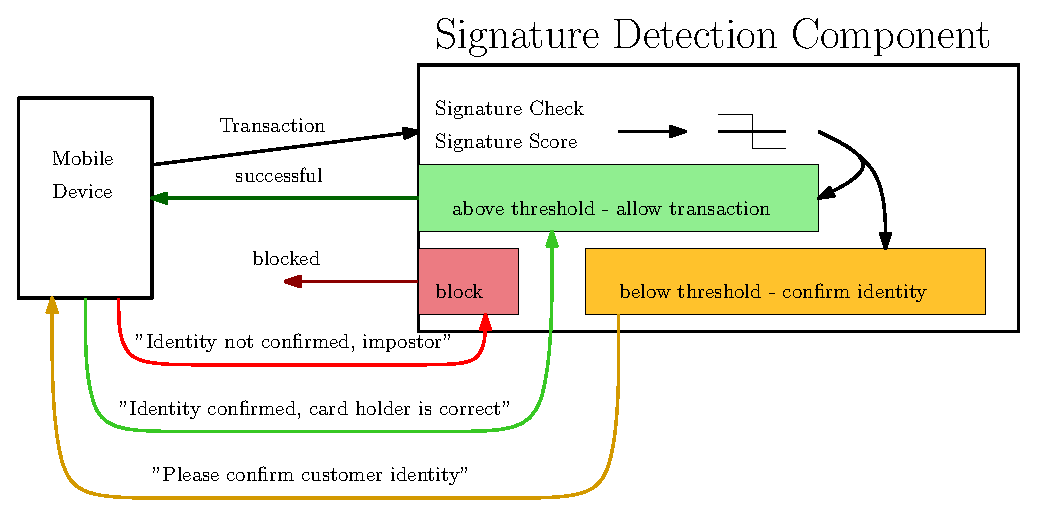
\includegraphics[width=1\textwidth]{figures/fb-loop2.eps}
    \end{center}
    \caption{Simplified illustration of processing a transaction with the feedback loop. If the signature check does not reach the acceptance level, a request is sent to the merchant to confirm the card holder's signature. After a positive confirmation, the transaction is processed, otherwised blocked.}
    \label{fig:fb-loop2}
\end{figure}













%%%%%%%%%%%%%%%%%%%%%%%%%%%%%%%%%%%%%%%% CHAPTER EXPERIMENTS
\chapter{Implementation and Evaluation}
\label{chp:experiments}
% offline vs online
% using dynamic features: speed, acceleration


% Circle Detection?
% X Detection?

Section \ref{sec:exp-preventive} will give insight into how our work has affected the number of false positives and thus the manual inputs from Operations have changed since the new component was released.

Section \ref{sec:exp-reactive} will first introduce the database of signatures we collected to test our signature verification algorithms and afterwards show the equal error rate (EER) achieved in different scenarios.


\section{Preventive Fraud Detection}
\label{sec:exp-preventive}

The algorithms described in Listing \ref{lst:world-check-parse} and Listing \ref{lst:world-check-lookup} were implemented in a Ruby Sinatra app with a REST interface and released to production about 2 months prior to the submission of this thesis.

\subsection{Setup}

The full database was parsed on a testing environment and the resulting data was copied over into production. The daily updates are received on the production machine and directly parsed into the production database through the parsing script.

The PEP/HRA check is performed either automatically or manually:
\begin{itemize}
\item \textbf{Automatically} for each new user during sign-up
\item \textbf{Automatically} for each existing user once a week to re-check each account after incorporating the changes of that week
\item \textbf{Manually} from the Operations Admin Panel (OAP) via a button
\end{itemize}

Each request must be triggered via a POST request. Depending on the user object that needs to be checked, the body of the request changes. Table \ref{tbl:har-pep-requests} lists the different request types.

\begin{table}[tb]
    \begin{center}
        \begin{tabular}{p{1.75cm}|p{3cm}p{7cm}}
        \hline
        \textbf{Method} & \textbf{Path} & \textbf{Parameter} \\
        \hline
        POST & /person/check & \{"params": \{"user\_id": "1"\}\} \\ \hdashline[0.5pt/3pt]
        POST & /person/check & \{"params": \{"business\_owner\_id": "1"\}\} \\ \hdashline[0.5pt/3pt]
        POST & /person/check & \{"params": \{"business\_officer\_id": "1"\}\} \\
        \hline
        \end{tabular}
    \end{center}
    \label{tbl:har-pep-requests}
    \caption{The requests received by the PEP/HAR component}
\end{table}

\subsection{Results}

The new component was released to production on March 4th, 2013, at beginning of calendar week 10. At the same time, the old component was discontinued. Every new user was automatically checked during the sign-up process. In addition to that, Business Officers and Owners were checked manually through SOAP by the Operations Team.

As SumUp is still growing rapidly, all numbers were normalized in respect to 1000 sign ups per week. The number of manual work could be greatly reduced. Chart \ref{fig:pep-hra-charts} shows how the number of matches reduced in calendar week 10 after the new component was released.
Due to high amount of manual work that was required to reject or approve a match, the false positives were often only rejected one or two week after the initial match, which explains the shift between the curves in Figure \ref{fig:pep-hra-charts}.

Typically, about 50 to 100 matches were generated per 1000 new users with the old component. Almost all of those were false positives and therefore cause manual work that wouldn't have been necessary. With the new component, we were able to drastically reduce the amount of manual work required. After introduction of the new check to the system, the typical amount of matches per 1000 new sign ups after the release of the new component is below 10. The peak in calendar week 14 was caused by a system migration where a lot of accounts were checked again. However, as these accounts had been previously rejected, they did not cause any additional manual work.

Umformulieren! die ration muss kleiner werden!!!
It is too early to say whether the ratio of false positives per matches was also significantly reduced due to the backlog of false positives that were cleared within the first weeks after the new component's release. However, the numbers in Table \ref{tbl:hra-pep-results} indicate a trend towards a lower amount of false positives per total amount of matches.

\begin{table}[tb]
    \begin{center}
        \begin{tabular}{cc|c|c|c}
        & week  & Matches   & False Positives   & Ratio \\ \cline{2-5}
\multirow{6}{*}{
\begin{sideways}
after release
\end{sideways}
}  & 13-15 & 3,29      & 1,39              & 42\%  \\ \cdashline{2-5}[0.5pt/3pt]
       & 13-14 & 25,36     & 1,40              & 6\%   \\ \cdashline{2-5}[0.5pt/3pt]
       & 13-13 & 1,77      & 0,98              & 56\%  \\ \cdashline{2-5}[0.5pt/3pt]
       & 13-12 & 2,84      & 0,95              & 33\%  \\ \cdashline{2-5}[0.5pt/3pt]
       & 13.11 & 2,20      & 2,42              & 110\% \\ \cdashline{2-5}[0.5pt/3pt]
       & 13-10 & 2,64      & 6,71              & 255\% \\ \cline{2-5}\cline{2-5}
\multirow{6}{*}{
\begin{sideways}
before release
\end{sideways}
       }  & 13-09 & 64,33     & 58,91             & 92\%  \\ \cdashline{2-5}[0.5pt/3pt]
       & 13-08 & 60,71     & 53,99             & 89\%  \\ \cdashline{2-5}[0.5pt/3pt]
       & 13-07 & 55,89     & 55,89             & 100\% \\ \cdashline{2-5}[0.5pt/3pt]
       & 13-06 & 77,83     & 77,83             & 100\% \\ \cdashline{2-5}[0.5pt/3pt]
       & 13-05 & 65,10     & 36,86             & 57\%  \\ \cdashline{2-5}[0.5pt/3pt]
       & 13-04 & 71,00     & 68,73             & 97\%  \\ \cline{2-5}
        \end{tabular}
    \end{center}
    \label{tbl:hra-pep-results}
    \caption{The requests received by the PEP/HAR component. Ratio: Erwaehnen von backlog! false positive beinhalten backlog}
\end{table}

\begin{figure}
        \centering
        \begin{subfigure}[b]{\textwidth}
                \centering
                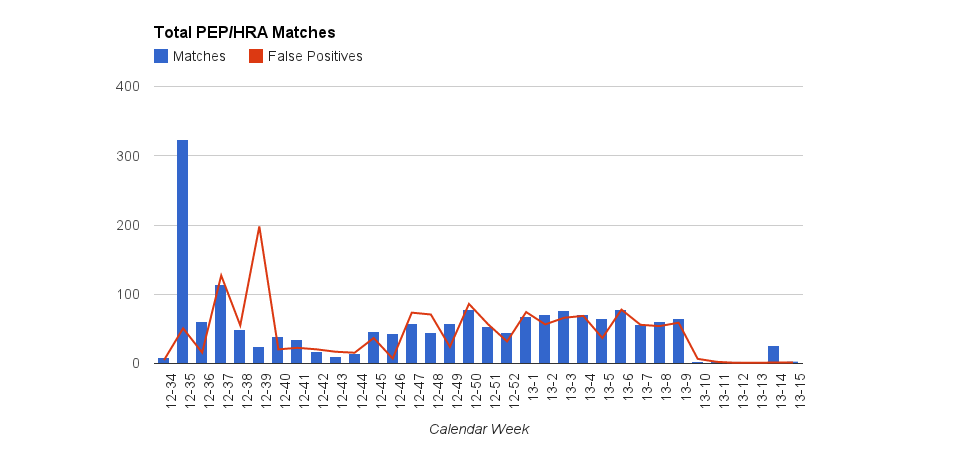
\includegraphics[width=\textwidth]{figures/chart_total.png}
                % \caption{HMM1}
                \label{fig:chart-total}
        \end{subfigure}%

        \begin{subfigure}[b]{\textwidth}
                \centering
                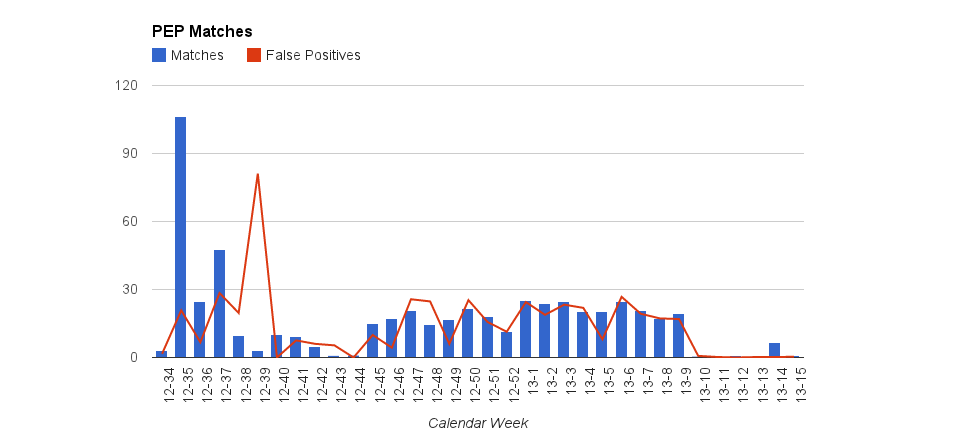
\includegraphics[width=\textwidth]{figures/chart_pep.png}
                % \caption{HMM1}
                \label{fig:chart-pep}
        \end{subfigure}%

        ~ %add desired spacing between images, e. g. ~, \quad, \qquad etc.
          %(or a blank line to force the subfigure onto a new line)
        \begin{subfigure}[b]{\textwidth}
                \centering
                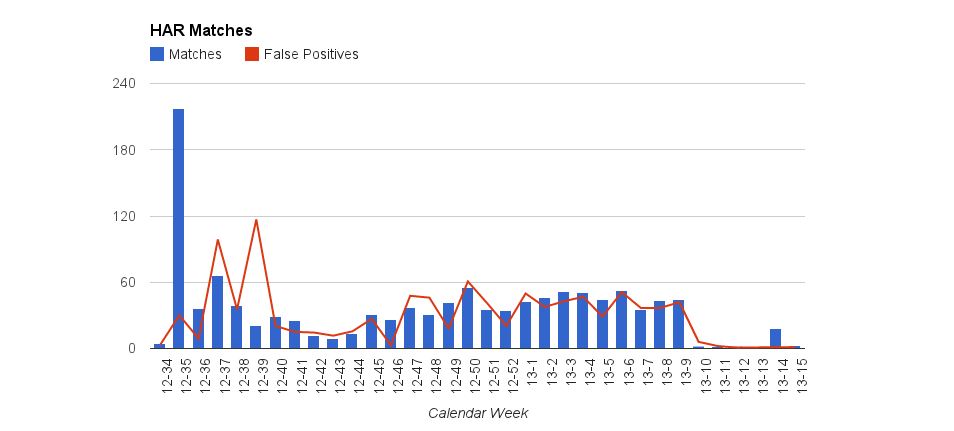
\includegraphics[width=\textwidth]{figures/chart_har.png}
                % \caption{HMM1}
                \label{fig:chart-har}
        \end{subfigure}%

        \caption{Evolution of the number of matches generated by the automatic PEP/HRA check. The top graph shows the evolution of the overall matches and false positives and the bottom and bottom graph the evolution for PEP and HRA separately. The new check was released to production in week 13-10 which is clearly visible as a drop in numbers.}
        \label{fig:pep-hra-charts}
\end{figure}

The operation department reports that the number of man hours was reduced since the release of the new component. It is still early but the numbers in Table \ref{tbl:man-hours} indicate that one to two full days of manual work were saved by introducing the new component.

Erwaehnen dass es absolute Zahlen sind in der Tabelle!

\begin{table}[tb]
    \begin{center}
        \begin{tabular}{c|c|c}Month & Matches (absolute numbers) & Man Hours \\ \hline
        December & 283 & 10 hours \\ \hdashline[0.5pt/3pt]
        January & 463 & 16 hours  \\ \hdashline[0.5pt/3pt]
        February & 853 & 29 hours \\ \hline \hline
        March & 125 & 4 hours \\ \hdashline[0.5pt/3pt]
        April (month to date) & 9 & 0.3 hours \\ \hline
        \end{tabular}
    \end{center}
    \label{tbl:man-hours}
    \caption{The requests received by the PEP/HAR component}
\end{table}



\section{Reactive Fraud Detection}
\label{sec:exp-reactive}

\subsection{Database}

As there don't seem to be any publicly available databases of signatures that were collected with a finger on a mobile device, we collected our own database and forgeries.
Between 8 and 80 Signatures per person were collected from 11 people on 4 different days on four different devices. This is an approximation of the reality in terms of how many signatures we have for one card holder and on how many different devices signatures for one card holder were collected. In total, a set of 487 signatures was collected. However, for most of our results, the signatures captured on the Android device were neglected due to a bug in the capturing software.
The devices used to collect the signatures are listed in Table \ref{tbl:signatures-devices} and were all used equally often.

\begin{table}[tb]
    \begin{center}
        \begin{tabular}{p{1.75cm}|p{2cm}p{2cm}p{2cm}p{2cm}}
        \hline

        \hline
        \textbf{Device} & \textbf{Software Version} & \textbf{Screen Size [cm]} & \textbf{Screen Resolution [px]} & \textbf{Pixel Density [ppi]} \\
        \hline
        Apple iPhone 4s & iOS 6.1.2 & 8.9 & 640x960 & 326 \\
        \hdashline[0.5pt/3pt]
        Apple iPhone 5 & iOS 6.1.2 & 10 & 640x1136 & 326 \\
        \hdashline[0.5pt/3pt]
        Samsung Galaxy Note II & Android 4.1.1 & 14.1 & 720x1280 & 267 \\
        \hdashline[0.5pt/3pt]
        Apple iPad mini & iOS 6.1.2 & 20 & 768x1024 & 163\\
        \hline
        \end{tabular}
    \end{center}
    \label{tbl:signatures-devices}
    \caption{The four devices used to collect signatures, ordered by screen size}
\end{table}

We also collected three forgeries for each person. The forgeries are created by an untrained person and of the following kind:

\begin{itemize}
\item \textbf{Spontaneous Forgery $\mathcal{F}_1$}: A random signature from the set of one person's signatures was shown the imposter for 5 secs. The imposter was only allowed to forge the signature after the five seconds.
\item \textbf{Sample Forgery $\mathcal{F}_2$}: A random signature from the set of one person's signatures was shown to the imposter for an indefinite amount of time and the imposter was able to look at the signature while forging the signature.
\item \textbf{Knowledgable Forgery $\mathcal{F}_3$}: The imposter had unlimited access to all of one person's signatures to forge the signature.
\end{itemize}

With each technique in our work, we gatheres statistics about two use cases:
\begin{itemize}
\item \textbf{Classification of signatures}: Our goal is to measure how well the algorithm performs in connecting a signature with its card holder. This part runs the ground truth agains itself.
\item \textbf{Detection of forgeries}: Our goal is to measure how well the algorithm is at detecting forgeries. The set of forgeries is run against this perticular card holder's set of confirmed signatures.
\end{itemize}

\subsection{Pre-Alignment and Normalization}

In order to compare the signatures, we normalized some of the properties before comparing the signatures.
\begin{itemize}
\item \textbf{Sampling rate}: Because we collected the signatures on touchscreen devices with event-based sampling, we got very different sampling rates. In order to compare signatures, we normalize the sampling rate to 20 Hz for all signatures, what is about half of the typical sampling of a signature which is collected on an iPhone 4s.
\item \textbf{Size and length}: The different screen size and pixel density between the devices caused very different height, width and length for the signatures. In order to compare them, we normalized the signatures height and width. Of course, when we used the width-to-height ratio as a global feature, we collected this value before normalization.
\item \textbf{Time}: As more screen estate also means longer distances to draw a signature, we also adjusted the timestamps when we normalized the size of a signature.
\end{itemize}








\subsection{Global Features}
Our solution uses the following global features, as listed in Section \ref{sec:features}:

\begin{itemize}
\item Signature length in pixels $l$
\item Total time to sign in milliseconds $t$
\item Maximum and average velocity $v_\text{max}, \bar{v}$
\item Maximum acceleration $a_\text{max}$
\item Number of segments $n$
\item Width to height ration $r$
\end{itemize}

Other common features, e.g.\ the total number of dots recorded, are irrelevant for our experiments as those features are device specific and can thus not be used to calculate the similarity between signatures.
Table \ref{tbl:global-features-results-avg} shows our results for the average of these features for each person's signature set.

\begin{figure}
    \centering
    \begin{subfigure}[b]{\textwidth}
            \centering
            \small
            \begin{tabular}{c|c|c|c|c|c|c|c}
            \hline
            \textbf{Person} & $l$ & $t$ & $v_\text{max}$ & $\bar{v}$ & $a_\text{max}$ & $n$ & $r$\\
            \hline
            0 & 1316.81 & 1640.0 & 2.27 & 0.8 & 1.11 & 2.0 & 0.0 \\ \hdashline[0.5pt/3pt]
            1 & 827.09 & 1373.0 & 1.5 & 0.6 & 0.58 & 2.0 & 1.0 \\ \hdashline[0.5pt/3pt]
            2 & 839.37 & 1445.0 & 1.71 & 0.58 & 0.7 & 2.0 & 2.0 \\ \hdashline[0.5pt/3pt]
            3 & 1434.08 & 2250.0 & 2.22 & 0.64 & 1.49 & 3.0 & 2.0 \\ \hdashline[0.5pt/3pt]
            4 & 669.82 & 1122.0 & 1.79 & 0.6 & 0.49 & 1.0 & 2.0 \\ \hdashline[0.5pt/3pt]
            5 & 924.78 & 1856.0 & 1.14 & 0.5 & 0.64 & 2.0 & 2.0 \\ \hdashline[0.5pt/3pt]
            6 & 1281.41 & 1399.0 & 2.49 & 0.92 & 1.53 & 2.0 & 1.0 \\ \hdashline[0.5pt/3pt]
            7 & 843.17 & 1424.0 & 1.13 & 0.59 & 0.48 & 2.0 & 1.0 \\ \hdashline[0.5pt/3pt]
            8 & 639.14 & 1209.0 & 1.7 & 0.53 & 0.73 & 1.0 & 1.0 \\ \hdashline[0.5pt/3pt]
            9 & 1299.5 & 5467.0 & 0.79 & 0.24 & 0.41 & 4.0 & 1.0 \\
            \hline
            \end{tabular}
            \label{tbl:global-features-results-min}
            \caption{The minimum values for each signature set and all global features}
    \end{subfigure}%

    \begin{subfigure}[b]{\textwidth}
            \centering
            \small
            \begin{tabular}{c|c|c|c|c|c|c|c}
            \hline
            \textbf{Person} & $l$ & $t$ & $v_\text{max}$ & $\bar{v}$ & $a_\text{max}$ & $n$ & $r$\\
            \hline
            0 & 1701.69 & 1942.75 & 15.5 & 0.88 & 16.93 & 2.13 & 0.5 \\ \hdashline[0.5pt/3pt]
            1 & 1235.27 & 1773.95 & 11.24 & 0.7 & 13.36 & 2.0 & 1.93 \\ \hdashline[0.5pt/3pt]
            2 & 1206.72 & 1762.06 & 10.22 & 0.68 & 18.96 & 3.11 & 2.33 \\ \hdashline[0.5pt/3pt]
            3 & 2565.76 & 3217.96 & 17.62 & 0.8 & 27.72 & 5.58 & 2.42 \\ \hdashline[0.5pt/3pt]
            4 & 1104.21 & 1588.11 & 8.1 & 0.7 & 9.58 & 3.43 & 2.81 \\ \hdashline[0.5pt/3pt]
            5 & 1308.19 & 3047.47 & 5.23 & 0.43 & 8.25 & 8.0 & 2.3 \\ \hdashline[0.5pt/3pt]
            6 & 2480.3 & 2102.87 & 13.71 & 1.18 & 16.89 & 3.87 & 2.04 \\ \hdashline[0.5pt/3pt]
            7 & 1260.28 & 2194.41 & 6.79 & 0.57 & 9.41 & 2.64 & 2.07 \\ \hdashline[0.5pt/3pt]
            8 & 1311.1 & 1574.98 & 11.18 & 0.83 & 15.12 & 2.6 & 1.47 \\ \hdashline[0.5pt/3pt]
            9 & 2047.7 & 6953.81 & 3.95 & 0.29 & 5.04 & 12.19 & 2.4 \\
            \hline
            \end{tabular}
            \label{tbl:global-features-results-avg}
            \caption{The average values for each signature set and all global features}
    \end{subfigure}%

    ~ %add desired spacing between images, e. g. ~, \quad, \qquad etc.
      %(or a blank line to force the subfigure onto a new line)
    \begin{subfigure}[b]{\textwidth}
            \centering
            \small
            \begin{tabular}{c|c|c|c|c|c|c|c}
            \hline
            \textbf{Person} & $l$ & $t$ & $v_\text{max}$ & $\bar{v}$ & $a_\text{max}$ & $n$ & $r$\\
            \hline
            0 & 2571.75 & 2282.0 & 54.42 & 1.13 & 73.35 & 3.0 & 1.0 \\ \hdashline[0.5pt/3pt]
            1 & 2048.9 & 2957.0 & 82.49 & 0.69 & 139.0 & 2.0 & 3.0 \\ \hdashline[0.5pt/3pt]
            2 & 2069.97 & 2117.0 & 52.35 & 0.98 & 105.95 & 5.0 & 3.0 \\ \hdashline[0.5pt/3pt]
            3 & 4673.42 & 9370.0 & 104.48 & 0.5 & 180.54 & 8.0 & 4.0 \\ \hdashline[0.5pt/3pt]
            4 & 2041.9 & 2914.0 & 63.79 & 0.7 & 99.93 & 5.0 & 4.0 \\ \hdashline[0.5pt/3pt]
            5 & 2425.82 & 4694.0 & 41.11 & 0.52 & 48.09 & 11.0 & 4.0 \\ \hdashline[0.5pt/3pt]
            6 & 4388.68 & 3633.0 & 75.89 & 1.21 & 134.83 & 5.0 & 3.0 \\ \hdashline[0.5pt/3pt]
            7 & 1958.88 & 4349.0 & 65.51 & 0.45 & 92.97 & 8.0 & 3.0 \\ \hdashline[0.5pt/3pt]
            8 & 2146.82 & 2749.0 & 65.46 & 0.78 & 112.3 & 4.0 & 2.0 \\ \hdashline[0.5pt/3pt]
            9 & 3428.25 & 8083.0 & 20.12 & 0.42 & 33.69 & 17.0 & 9.0 \\
            \hline
            \end{tabular}
            \label{tbl:global-features-results-max}
            \caption{The maximum values for each signature set and all global features}
    \end{subfigure}%

    \caption{The minimum, average and maximum values we obtained for all global features for each subject's set of signatures.}
    \label{fig:global-features}
\end{figure}

\noindent\textbf{Similarity score $S_{GF}$}\\
We use our knowledge about the minimum, average and maximum value for each of the sigature sets for a specific card holder to create a similarity score.
We compute the seven global features for a test signature and we assign a point for each of the features if the test value lies between the minimum and maximum that we computed earlier. This gives us the score vector
$$G = [s_l, s_t, s_{v_\text{max}}, s_{\bar{v}}, s_{a_\text{max}}, s_n, s_r]$$

We assume that not all of the global features are of the same significance. We therefore define a  weigthing vector $$W = [w_l, w_t, w_{v_\text{max}}, w_{\bar{v}}, w_{a_\text{max}}, w_n, w_r]$$

Our similarity score is calculated as
$$S_{GF} = G \times W$$

As this approach includes every signature every collected and thereby possibly enlarges the windows where other signatures are matched, a sliding window should be used for larger datasets. As we were are working with less than 30 signatures per card holder, we did not implement a sliding window mechanism for this work.

\noindent\textbf{Fitness function $\mathbb{F}_{GF}$}\\
We run each signature against each of the eleven signature models, defined by global features maxima and minima of a system. The fitness function tries to reduce the number of signatures which receive the highes possible similarity score for a given weighting vector $W$.
As all signatures will score a perfect score at least once, the fitness function's goal is to come as close to the number of signatures in the ground truth set as possible.

The definition of $\mathbb{F}$ is given in pseudo code in Listing \ref{lst:global-features-fitness-function}.


\begin{lstlisting}[caption={The fitness function for global features tries to reduce the number of signatures with the hightes possible score for a given weighting vector $W$},label={lst:global-features-fitness-function}]

until fitness == #signatures_in_groundtruth

    fitness = calculate_globabl_features w

    if fitness < previous_fitness
        save w
    end

    permutate w
end
\end{lstlisting}


\noindent\textbf{Classification of Signatures}\\
We defined the start vecor $W = [0,0,0,0,0,0,0]$ and let the fitness function permutate the vector until a local minimum was found for all $W$ consisting of $\{0,1,2\}$. The local minima was reached for $$W = [w_l, w_t, w_{v_\text{max}}, w_{\bar{v}}, w_{a_\text{max}}, w_n, w_r] = [0, 1, 0, 1, 0, 1, 1]$$
At the local minimum, there are 755 signatures with the highest score which is 478 more than in the ground truth (278) that we used for this approach.

We conclude that time $t$, average velocity $\bar{v}$, the number of segments $n$ and the width-to-height ratio $r$ should be used to compare signatures.

If we extend our search and include the two groups with the highest occurrences, we get still get 840 signatures included in the highest and second highest score and the weighting vector:
$$W = [w_l, w_t, w_{v_\text{max}}, w_{\bar{v}}, w_{a_\text{max}}, w_n, w_r] = [0, 2, 0, 2, 0, 2, 1]$$


\noindent\textbf{Detection of forgeries}\\
We used the previously found vector to test the robustness of this approach against forgeries. We set $$W = [0, 1, 0, 1, 0, 1, 1]$$
and ran all the forgeries against the previously trained signature models given by the minimum and maximum values.

We computed these four values for each of the found global features, $t, \bar{v}, n$ and $r$. We then checked whether they lie within the bounds for that feature for each person. The results can be seen in Figure \ref{fig:global-features-forgeries}. The tables first list the min/max for each feature, the value found for the forgery and whether or not it was a hit.

A hit means that the test value lies within the reference min/max for all four features.
We notice that most of the matches were falsified mostly because the impostor took too long to sign ($t$ too high) or because he didn't sign fast enough ($\bar{v}$ too little). Out of the 30 forgeries, only one of the simple forgeries was a hit. This corresponds to an error rate of 3.33 percent.

\noindent\textbf{Computational complexity}\\
Computing the features for a signature and comparing them to the previously computed min/max values takes less than a tenth of a second and the approach is therefore feasible in realtime. In addition, by using a sliding window, the computational complexity of computing the min/max values will stay at a predictable level even though the total signature set may grow very large.

\begin{figure}
    \centering
    \begin{subfigure}[b]{\textwidth}
            \centering
            \tabcolsep 4pt
            \small
            \begin{tabular}{c|cccc||cccc||c}
            \hline
            \textbf{P} & $t_r$ & $\bar{v}_r$ & $n_r$ & $r_r$ & $t_f$ & $\bar{v}_f$ & $n_f$ & $r_f$ & Hit \\
            \hline
            0 & [1640.0, 2282.0] & [0.8, 1.13] & [2.0, 3.0] & [0.0,1.0] & 13782.0 & 0.14 & 2.0 & 2.0 & \xmark \\ \hdashline[0.5pt/3pt]
            1 & [1373.0, 2957.0] & [0.6, 0.69] & [2.0, 2.0] & [1.0,3.0] & 5229.0 & 0.29 & 1.0 & 2.0 & \xmark\\ \hdashline[0.5pt/3pt]
            2 & [1445.0, 2117.0] & [0.58, 0.98] & [2.0, 5.0] & [2.0,3.0] & 4141.0 & 0.29 & 5.0 & 2.0 & \xmark\\ \hdashline[0.5pt/3pt]
            3 & [2250.0, 9370.0] & [0.5, 0.64] & [3.0, 8.0] & [2.0,4.0] & 3252.0 & 0.34 & 2.0 & 1.0 & \xmark \\ \hdashline[0.5pt/3pt]
            4 & [1122.0, 2914.0] & [0.6, 0.7] & [1.0, 5.0] & [2.0,4.0] & 8743.0 & 0.15 & 3.0 & 2.0 & \xmark \\ \hdashline[0.5pt/3pt]
            5 & [1856.0, 4694.0] & [0.5, 0.52] & [2.0, 11.0] & [2.0,4.0] & 3658.0 & 0.39 & 4.0 & 2.0 & \xmark \\ \hdashline[0.5pt/3pt]
            6 & [1399.0, 3633.0] & [0.92, 1.21] & [2.0, 5.0] & [1.0,3.0] & 2815.0 & 0.53 & 2.0 & 2.0 & \xmark \\ \hdashline[0.5pt/3pt]
            7 & [1424.0, 4349.0] & [0.59, 0.45] & [2.0, 8.0] & [1.0,3.0] & 3978.0 & 0.48 & 2.0 & 2.0 & \cmark \\ \hdashline[0.5pt/3pt]
            8 & [1209.0, 2749.0] & [0.53, 0.78] & [1.0, 4.0] & [1.0,2.0] & 10863.0 & 0.19 & 4.0 & 2.0 & \xmark \\ \hdashline[0.5pt/3pt]
            9 & [5467.0, 8083.0] & [0.24, 0.42] & [4.0, 17.0] & [1.0,9.0] & 24910.0 & 0.08 & 18.0 & 1.0 & \xmark \\ \hdashline[0.5pt/3pt]
            \hline
            \end{tabular}
            \label{tbl:global-features-forg-spontaneous}
            \caption{The results for spontaneous forgeries $\mathcal{F}_1$}
    \end{subfigure}%

    \begin{subfigure}[b]{\textwidth}
            \centering
            \tabcolsep 4pt
            \small
            \begin{tabular}{c|cccc||cccc||c}
            \hline
            \textbf{P} & $t_r$ & $\bar{v}_r$ & $n_r$ & $r_r$ & $t_f$ & $\bar{v}_f$ & $n_f$ & $r_f$ & Hit \\
            \hline
            0 & [1640.0, 2282.0] & [0.8, 1.13] & [2.0, 3.0] & [0.0,1.0] & 4477.0 & 0.38 & 3.0 & 1.0 & \xmark \\ \hdashline[0.5pt/3pt]
            1 & [1373.0, 2957.0] & [0.6, 0.69] & [2.0, 2.0] & [1.0,3.0] & 7835.0 & 0.22 & 2.0 & 1.0 & \xmark \\ \hdashline[0.5pt/3pt]
            2 & [1445.0, 2117.0] & [0.58, 0.98] & [2.0, 5.0] & [2.0,3.0] & 10237.0 & 0.16 & 5.0 & 1.0 & \xmark \\ \hdashline[0.5pt/3pt]
            3 & [2250.0, 9370.0] & [0.5, 0.64] & [3.0, 8.0] & [2.0,4.0] & 11261.0 & 0.17 & 3.0 & 1.0 & \xmark \\ \hdashline[0.5pt/3pt]
            4 & [1122.0, 2914.0] & [0.6, 0.7] & [1.0, 5.0] & [2.0,4.0] & 5508.0 & 0.2 & 3.0 & 3.0 & \xmark \\ \hdashline[0.5pt/3pt]
            5 & [1856.0, 4694.0] & [0.5, 0.52] & [2.0, 11.0] & [2.0,4.0] & 2465.0 & 0.54 & 3.0 & 2.0 & \xmark \\ \hdashline[0.5pt/3pt]
            6 & [1399.0, 3633.0] & [0.92, 1.21] & [2.0, 5.0] & [1.0,3.0] & 7338.0 & 0.22 & 2.0 & 1.0 & \xmark \\ \hdashline[0.5pt/3pt]
            7 & [1424.0, 4349.0] & [0.59, 0.45] & [2.0, 8.0] & [1.0,3.0] & 9386.0 & 0.19 & 2.0 & 2.0 & \xmark \\ \hdashline[0.5pt/3pt]
            8 & [1209.0, 2749.0] & [0.53, 0.78] & [1.0, 4.0] & [1.0,2.0] & 15633.0 & 0.1 & 8.0 & 2.0 & \xmark \\ \hdashline[0.5pt/3pt]
            9 & [5467.0, 8083.0] & [0.24, 0.42] & [4.0, 17.0] & [1.0,9.0] & 11826.0 & 0.12 & 16.0 & 2.0 & \xmark \\ \hdashline[0.5pt/3pt]
            \hline
            \end{tabular}
            \label{tbl:global-features-forg-sample}
            \caption{The results for sample forgeries $\mathcal{F}_2$}
    \end{subfigure}%

    \begin{subfigure}[b]{\textwidth}
            \centering
            \tabcolsep 4pt
            \small
            \begin{tabular}{c|cccc||cccc||c}
            \hline
            \textbf{P} & $t_r$ & $\bar{v}_r$ & $n_r$ & $r_r$ & $t_f$ & $\bar{v}_f$ & $n_f$ & $r_f$ & Hit \\
            \hline
            0 & [1640.0, 2282.0] & [0.8, 1.13] & [2.0, 3.0] & [0.0,1.0] & 10799.0 & 0.16 & 2.0 & 2.0 & \xmark \\ \hdashline[0.5pt/3pt]
            1 & [1373.0, 2957.0] & [0.6, 0.69] & [2.0, 2.0] & [1.0,3.0] & 3896.0 & 0.55 & 2.0 & 2.0 & \xmark \\ \hdashline[0.5pt/3pt]
            2 & [1445.0, 2117.0] & [0.58, 0.98] & [2.0, 5.0] & [2.0,3.0] & 9016.0 & 0.27 & 4.0 & 2.0 & \xmark \\ \hdashline[0.5pt/3pt]
            3 & [2250.0, 9370.0] & [0.5, 0.64] & [3.0, 8.0] & [2.0,4.0] & 6731.0 & 0.24 & 2.0 & 2.0 & \xmark \\ \hdashline[0.5pt/3pt]
            4 & [1122.0, 2914.0] & [0.6, 0.7] & [1.0, 5.0] & [2.0,4.0] & 5506.0 & 0.29 & 2.0 & 2.0 & \xmark \\ \hdashline[0.5pt/3pt]
            5 & [1856.0, 4694.0] & [0.5, 0.52] & [2.0, 11.0] & [2.0,4.0] & 3442.0 & 0.41 & 3.0 & 2.0 & \xmark \\ \hdashline[0.5pt/3pt]
            6 & [1399.0, 3633.0] & [0.92, 1.21] & [2.0, 5.0] & [1.0,3.0] & 9328.0 & 0.17 & 2.0 & 1.0 & \xmark \\ \hdashline[0.5pt/3pt]
            7 & [1424.0, 4349.0] & [0.59, 0.45] & [2.0, 8.0] & [1.0,3.0] & 6295.0 & 0.26 & 2.0 & 2.0 & \xmark \\ \hdashline[0.5pt/3pt]
            8 & [1209.0, 2749.0] & [0.53, 0.78] & [1.0, 4.0] & [1.0,2.0] & 7133.0 & 0.24 & 6.0 & 2.0 & \xmark \\ \hdashline[0.5pt/3pt]
            9 & [5467.0, 8083.0] & [0.24, 0.42] & [4.0, 17.0] & [1.0,9.0] & 9138.0 & 0.17 & 17.0 & 2.0 & \xmark \\ \hdashline[0.5pt/3pt]
            \hline
            \end{tabular}
            \label{tbl:global-features-forg-knowledgable}
            \caption{The results for knowledgable forgeries $\mathcal{F}_3$}
    \end{subfigure}%


    \caption{The minimum, average and maximum values we obtained for all global features for each subject's set of signatures.}
    \label{fig:global-features-forgeries}
\end{figure}



% Findings:
% -ration is a very weak indicator
% - v_avg is ok
% - vmax weak
% - amax weak

\subsection{Dynamic Time Warping}

\noindent\textbf{Similarity score $S_{DTW}$}\\
The similarity score is given as the DTW's output.
We have evaluated two kinds of distances
\begin{itemize}
\item the 2-Norm of the $x,y$-vector
\item the 2-Norm of the $x,y,t$-vector which includes the timestamp for each point
\end{itemize}

We have tested combinations of the following inputs:
\begin{itemize}
\item \textbf{Age}: We do not use the full signature set for every card holder to reduce the computation time. We therefore choose a subset of signatures. We test recent signatures, i.e.\ chronologically the last 5, 10 or 20 signatures, or old signatures, i.e.\ the first 5, 10, 20 signatures ever recorded by a card holder.
\item \textbf{Amount of signatures}: For computation reasons we restrict the set of signatures to a subset. We obtain the results for 5, 10 and 20 signatures. We also run one full experiment with up to 50 signatures for each card holder.
\item \textbf{Lengh}: We noted that the variability of a signature is often higher towards the end than at the beginning and therefore perform experiments using the full, i.e.\ including all points of a signature, or only a subset, which we annotate as partial.
\item \textbf{Vector}: We calculate the distance between two points during the DTW algorithm as either between the geometric position $x,y$ or the geometric position including the time $x,y,t$.
\end{itemize}

\noindent\textbf{Fitness function $\mathbb{F}_{DTW}$}\\

The fitness function $\mathbb{F}_{DTW}$ is defined as the Equal Error Rate (EER) during the classification phase. It is used to determine the optimal threshold to accept/reject a signature.

We are also interested in the computation time to compute the EER to know whether or not a combination is feasible for real time evaluation.

\begin{table}
    \centering
    \tabcolsep 4pt
    \begin{tabular}{l|cccc|cccc|c}
    \hline
    Experiment & Age & \# Sig & Length & Vector & Time [s] & Threshold & EER\\
    \hline
         1 & recent & 5   & full      & xyt   & 249   & 0.02  & 0.29 \\ \hdashline[0.5pt/3pt] % 1366148189
         2 & recent & 5   & full      & xy    & 222   & 0.07  & 0.32 \\ \hdashline[0.5pt/3pt] % 1366148141
         3 \ref{fig:dtw-exp3} & recent & 5   & partial   & xyt   & 45    & 0.23  & 0.19 \\ \hdashline[0.5pt/3pt]
         4 \ref{fig:dtw-exp1} & recent & 5   & partial   & xy    & 40    & 0.30  & 0.12 \\ \hdashline[0.5pt/3pt] % 1366147505
         5 & recent & 10  & full      & xyt   & 782   & 0.02  & 0.33 \\ \hdashline[0.5pt/3pt] %1366146140
         6 & recent & 10  & full      & xy    & 762   & 0.06  & 0.29 \\ \hdashline[0.5pt/3pt] %1366146150
         7 & recent & 10  & partial   & xyt   & 189   & 0.22  & 0.29 \\ \hdashline[0.5pt/3pt] %1366146759
         8 \ref{fig:dtw-exp2} & recent & 10  & partial   & xy    & 171   & 0.30  & 0.14 \\ \hdashline[0.5pt/3pt]
         9 & recent & 20  & partial   & xyt   & 728   & 0.16  & 0.37 \\ \hdashline[0.5pt/3pt] % 1366149232
         10 & recent & 20  & partial   & xy    & 661   & 0.28  & 0.20 \\ \hdashline[0.5pt/3pt] % 1366149159
         11 & old & 10  & full      & xyt   & 944   & 0.01  & 0.39 \\ \hdashline[0.5pt/3pt] %1366151221
         12 & old & 10  & full      & xy    & 866   & 0.05  & 0.30 \\ \hdashline[0.5pt/3pt] %1366151125
         13 \ref{fig:dtw-exp4} & recent & 50 & partial & xy & 2137 & 0.26 & 0.33 \\ \hdashline[0.5pt/3pt] %1366153811

    \hline
    \end{tabular}
    \label{tbl:dtw-experiments1}\caption{Results of DTW experiments}
\end{table}

\noindent\textbf{Classification of Signatures}\\
The results of our experiments are listed in Figure \ref{tbl:dtw-experiments1}.
We found that:
\begin{itemize}
\item The algorithm performs better on distance vectors that exclude time information.
\item The algorithm is faster with less signatures per card holder and for a distance vector which excludes time information.
\item More recent signatures perform better than older signatures. This motivates the use of a sliding window.
\item Partial information of the signature vector is not only a lot faster but can also perform a lot better than full information. This is due to the higher variability in the signatures towards the end.
\item Signtaure classification in general is very time consuming and could not be done in real time.
\end{itemize}

The best performing combination is found to be
\begin{itemize}
\item Recent signatures
\item Five signatures per card holder
\item Partial information of the signature vector
\item No time information in the distance function
\end{itemize}

Experiment 4 produces an EER of 0.12 with a threshold of 0.3. Computing the similarity score $S_{DTW}$ for the cross product of all signatures took 40 seconds, which also makes it the fastes approach. The graphic representation is shown in Figure \ref{fig:dtw-exp1}. We use this setup to detect forgeries.


\begin{figure}
        \centering
        \begin{subfigure}[b]{\textwidth}
                \centering
                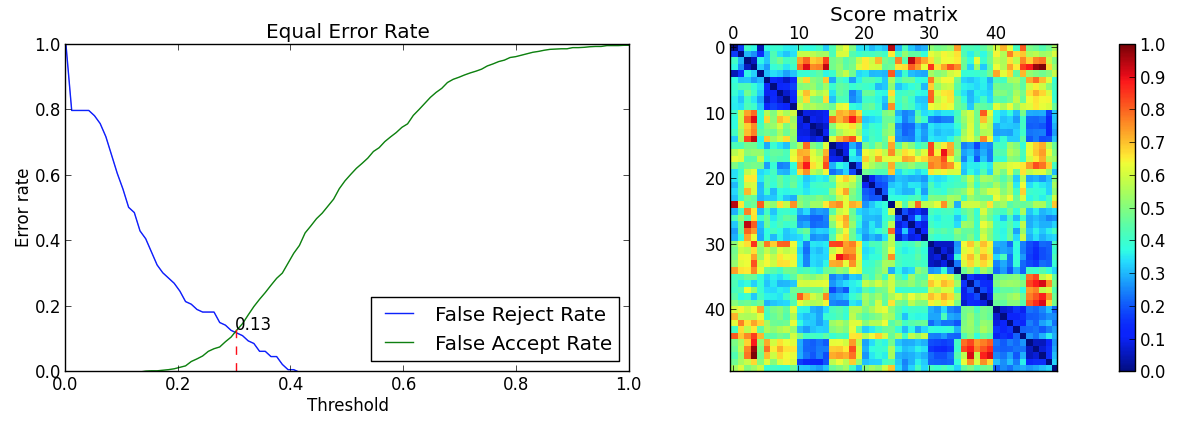
\includegraphics[width=0.8\textwidth]{figures/dtw-exp1.png}
                \caption{DTW with five recent signatures per card holder, partial information about each signature and excluding time information}
                \label{fig:dtw-exp1}
        \end{subfigure}%

        \begin{subfigure}[b]{\textwidth}
                \centering
                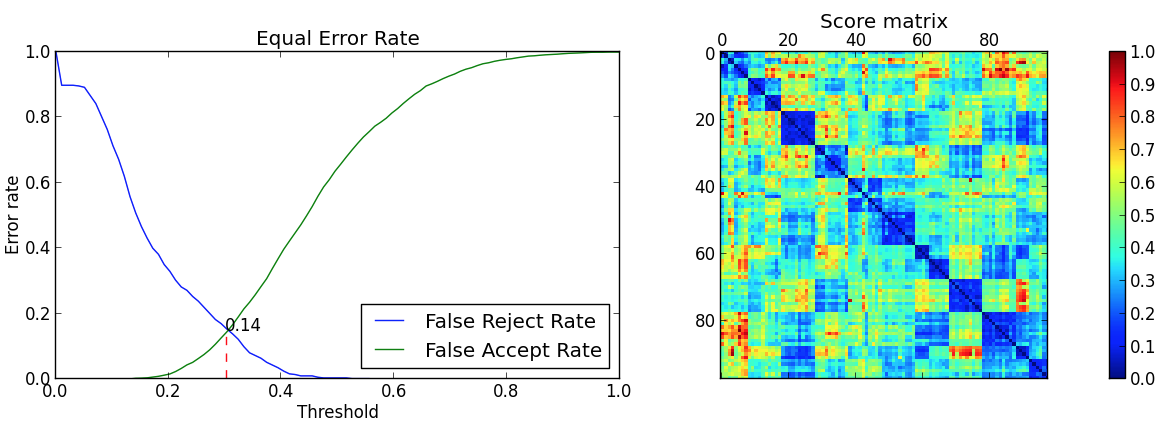
\includegraphics[width=0.8\textwidth]{figures/dtw-exp2.png}
                \caption{DTW with ten recent signatures per card holder, partial information about each signature and excluding time information}
                \label{fig:dtw-exp2}
        \end{subfigure}%

        ~ %add desired spacing between images, e. g. ~, \quad, \qquad etc.
          %(or a blank line to force the subfigure onto a new line)
        \begin{subfigure}[b]{\textwidth}
                \centering
                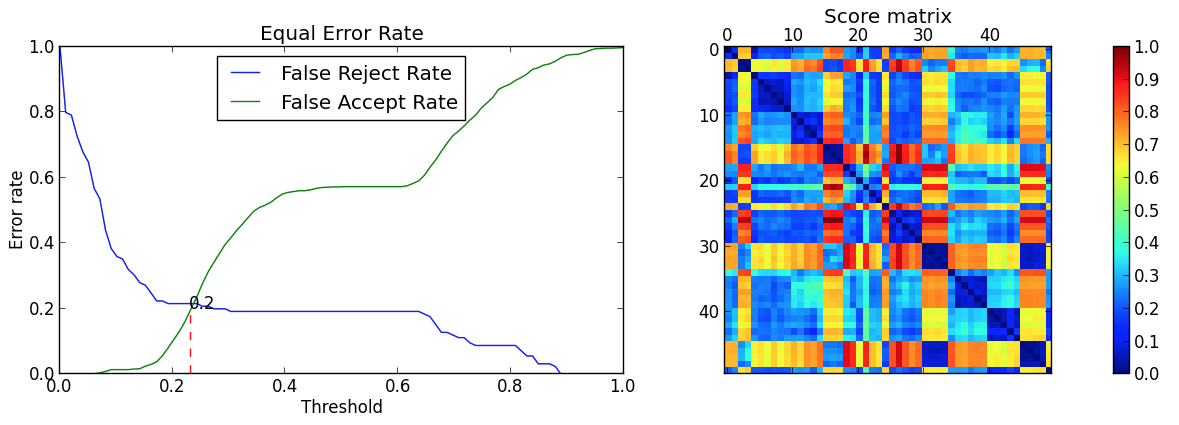
\includegraphics[width=0.8\textwidth]{figures/dtw-exp3.png}
                \caption{DTW with five recent signatures per card holder, partial information about each signature and including time information}
                \label{fig:dtw-exp3}
        \end{subfigure}%

        \begin{subfigure}[b]{\textwidth}
                \centering
                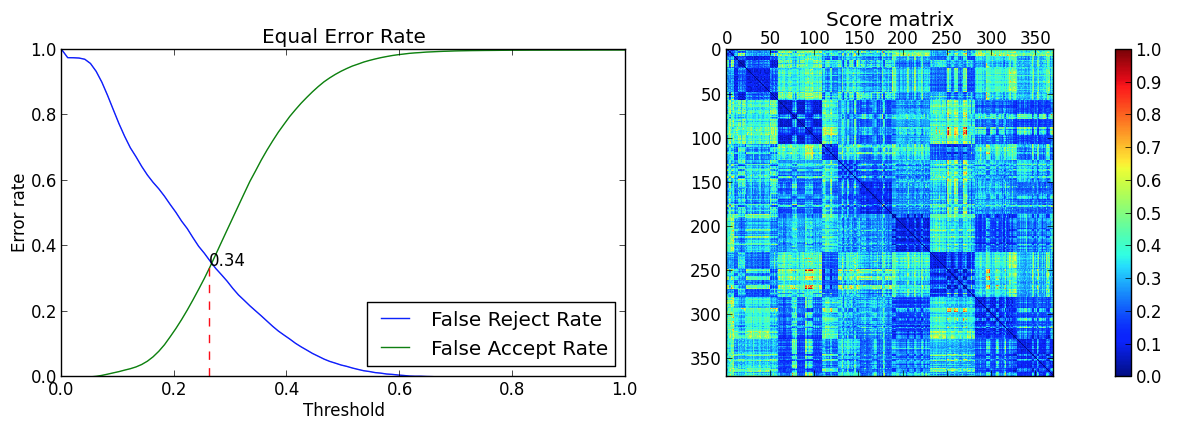
\includegraphics[width=0.8\textwidth]{figures/dtw-exp4.png}
                \caption{DTW with up to 50 recent signatures per card holder, partial information about each signature and excluding time information}
                \label{fig:dtw-exp3}
        \end{subfigure}%

        \caption{EER and Heatmap of the three best performing and the longtest DTW experiments}\label{fig:dtw-experiments2}
\end{figure}

\noindent\textbf{Detection of forgeries}\\
We calculate the distance between each forgery and each signature of a card holder's ground truth and use majority voting to decide whether a signature is accepted or rejected. The vote of two signatures counts as a positive vote if $S_{DTW}$ is higher than the found threshold of 0.30.

The maximum score we found in the previous experiment was 241881, the threshold of 0.3 therefore corresponds to $241881 \cdot 0.3 = 72564.2$.
In the 30 forgeries, we got 11 false positives as shown in Figure \ref{tbl:dtw-forgeries-results-tbl}. That corresponds to an error rate of 36 percent.



\begin{figure}
    \centering

    \begin{subfigure}[b]{0.3\textwidth}
            \centering
            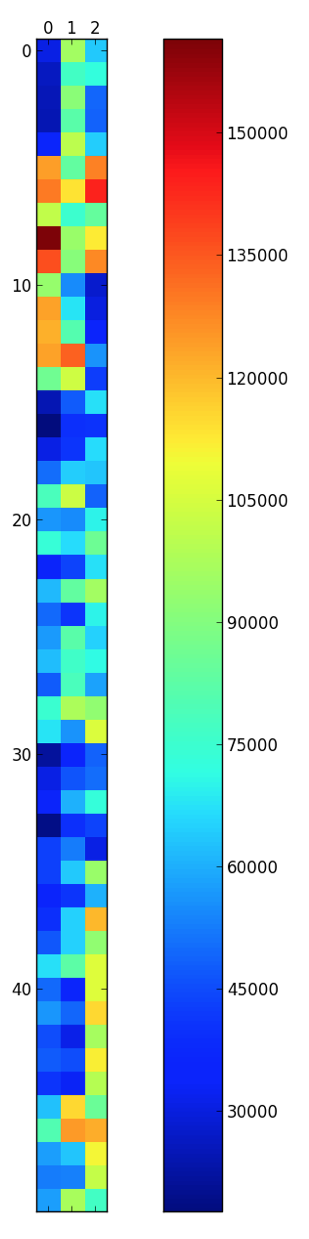
\includegraphics[width=0.8\textwidth]{figures/dtw_forgeries_1.png}
            \caption{}
            \label{fig:dtw-forgeries1}
    \end{subfigure}%
    \qquad
    \begin{subfigure}[b]{0.3\textwidth}
            \centering
            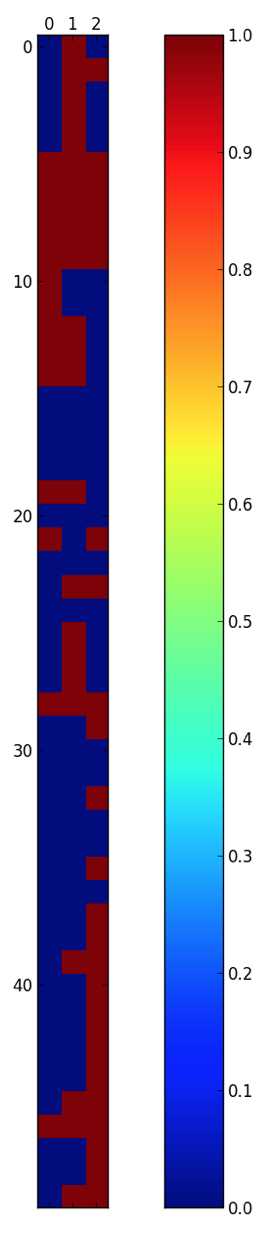
\includegraphics[width=0.8\textwidth]{figures/dtw_forgeries_2.png}
            \caption{}
            \label{fig:dtw-forgeries2}
    \end{subfigure}%
    \qquad
    \begin{subfigure}[b]{0.3\textwidth}
            \centering
            \tabcolsep 4pt
            \small
            \begin{tabular}{c|cccc||cccc||c}
            \hline
            \textbf{P} & $\mathcal{F}_1$ & $\mathcal{F}_2$ & $\mathcal{F}_3$ \\
            \hline
            1 & \xmark & \cmark & \xmark \\ \hdashline[0.5pt/3pt]
            2 & \cmark & \cmark & \cmark \\ \hdashline[0.5pt/3pt]
            3 & \cmark & \cmark & \xmark \\ \hdashline[0.5pt/3pt]
            4 & \xmark & \xmark & \xmark \\ \hdashline[0.5pt/3pt]
            5 & \xmark & \xmark & \xmark \\ \hdashline[0.5pt/3pt]
            6 & \xmark & \cmark & \xmark \\ \hdashline[0.5pt/3pt]
            7 & \xmark & \xmark & \xmark \\ \hdashline[0.5pt/3pt]
            8 & \xmark & \xmark & \cmark \\ \hdashline[0.5pt/3pt]
            9 & \xmark & \xmark & \cmark \\ \hdashline[0.5pt/3pt]
            10 & \xmark & \cmark & \cmark \\ \hdashline[0.5pt/3pt]
            \hline
            \end{tabular}
            \label{tbl:dtw-forgeries-results-tbl}
            \caption{}
    \end{subfigure}%



    \caption{The heatmap (a), the discretized heatmap after applying the threshold (b) and the false positives after applying majority voting (c)}
    \label{fig:dtw-forgeries-results}
\end{figure}




\noindent\textbf{Computational complexity}\\
Calculating the DTW score between two signatures takes about one tenth of a second on a modern computer which is by far fast enough to fulfill our real time requirements. However, computing the threshold requires longer computation and should be implemented in a background process.











\subsection{Hidden Markov Models}

There are several implementations of the HMM algorithm available. We found the implementation by MATLAB to be best documented and best fitting for our application and chose to work with said tool suite.

\noindent\textbf{Similarity score $S_{HMM}$}\\
After training the HMM for each card holder, we can calculate the likelihood for each signature to belong to a certain HMM. We define $S_{HMM}$ to be the likelihood of a signature to being generated by a certain model's card holder.

\noindent\textbf{Fitness function $\mathbb{F}_{HMM}$}\\

We want the range of likelihoods for each signature set against each signature model to be as small as possible. We therefore recorded the ranges in Table XX while we tested the system with five, six and seven states.
We vary the number of hidden states in the model as we try to minimize the window of likelihood for each signature set.

We calculate the window for each model and how many false positives we get in that case. We stopped our experiments at 9 states as it would otherwise become unfeasible to implement


\begin{table}
    \centering
    \tabcolsep 4pt
    \begin{tabular}{l|ccc|ccc}
    \hline
    Exp & States & \# Sig & Time [s] & Avg window size & False Positives / 100 Sig \\ \hline
    1 & 5 & 10 & 48                  & 142.0 & 16.63 \\ \hdashline[0.5pt/3pt]
    2 & 5 & 50 & 214                 & 209.0 & 33.8 \\ \hdashline[0.5pt/3pt]
    3 & 6 & 10 & 61                  & 144.0 & 12.45 \\ \hdashline[0.5pt/3pt]
    4 & 6 & 50 & 560                 & 593.0 & 44.18 \\ \hdashline[0.5pt/3pt]
    5 & 7 & 10 & 105                 & 144.0 & 9.8 \\ \hdashline[0.5pt/3pt]
    6 & 7 & 50 & 740                 & 370.0 & 34.72 \\ \hdashline[0.5pt/3pt]
    7 & 8 & 10 & 150                 & 145.0 & 7.14 \\ \hdashline[0.5pt/3pt]
    8 & 9 & 10 & 225                 & 148.0 & 5.1 \\ \hdashline[0.5pt/3pt]

    \hline
    \end{tabular}
    \label{tbl:hmm_experiments1}\caption{Results of HMM experiments}
\end{table}








\noindent\textbf{Classification of Signatures}\\
As shown in Table \ref{tbl:hmm_experiments1} the experiments with more signatures cause larger windows and thereby a higher number of false positives per 100 Sig.





\noindent\textbf{Detection of forgeries}\\
We decided to weight the lower computation time higher than the lower average of forgeries and performed the experiments on forgery detection with the parameters used for experiment 5:
\begin{itemize}
\item 7 hidden states
\item The model is trained with the 10 most recent signatures
\item The symbol alphabet consists of 8 angles
\end{itemize}

We obtain the window sizes in Table \ref{XX} for our experiments.

\begin{table}
    \centering
    \tabcolsep 4pt
    \begin{tabular}{l|ccc|ccc}
    \hline
    Exp & States & \# Sig & Time [s] & Avg window size & False Positives / 100 Sig \\ \hline
    1 & 5 & 10 & 48                  & 142.0 & 16.63 \\ \hdashline[0.5pt/3pt]
    2 & 5 & 50 & 214                 & 209.0 & 33.8 \\ \hdashline[0.5pt/3pt]
    3 & 6 & 10 & 61                  & 144.0 & 12.45 \\ \hdashline[0.5pt/3pt]
    4 & 6 & 50 & 560                 & 593.0 & 44.18 \\ \hdashline[0.5pt/3pt]
    5 & 7 & 10 & 105                 & 144.0 & 9.8 \\ \hdashline[0.5pt/3pt]
    6 & 7 & 50 & 740                 & 370.0 & 34.72 \\ \hdashline[0.5pt/3pt]
    7 & 8 & 10 & 150                 & 145.0 & 7.14 \\ \hdashline[0.5pt/3pt]
    8 & 9 & 10 & 225                 & 148.0 & 5.1 \\ \hdashline[0.5pt/3pt]

    \hline
    \end{tabular}
    \label{tbl:hmm_window_sizes}\caption{Results of HMM experiments}
\end{table}



\noindent\textbf{Computational complexity}\\

training with 6 states took 30s per model on average

computing the likelihood for a signature and a model takes less than a tenth of a second

% \subsection{Results}

% Computational feasibility

\subsection{Fusion of scores}

How correlated are the three scores?

Which tool can i use for this?

Wenn schlecht korreliert: Fusion ein guter Ansatz

Fusion-Techniken: 1/3 Score each oder 2 lowest oder 2 highest oder anderes weighting




% \subsection{Forgeries}
% A signature verification system typically focuses on the detection of one or more category of forged signatures. A skilled forgery is produced when the forger has unrestricted
% access to one or more samples of the writer’s actual signa- ture (see Figure 1b). A casual forgery or a simple forgery (see Figure 1c) is produced when the forger is familiar with the writer’s name, but does not have access to a sample of the ac- tual signature—stylistic differences are therefore prevalent. A random forgery or zero-effort forgery (see Figure 1d) can be any random scribble or a signature of another writer, and may even include the forger’s own signature. The genuine signatures and high quality forgeries for other writers are usually considered to be forgeries of this type.
% Skilled forgeries can be subdivided into amateur and pro- fessional forgeries. A professional forgery is produced by an in- dividual who has professional expertise in handwriting anal- ysis. They are able to circumvent obvious problems and ex- ploit their knowledge to produce high-quality, spacial forg- eries (see Figure 2b).

% In the context of online verification, amateur forgeries can be subdivided into home-improved and over-the-shoulder forgeries (see [6]). The category of home-improved forgeries contains forgeries that are produced when the forger has a paper copy of a genuine signature and has ample opportu- nity to practice the signature at home. Here the imitation is based only on the static image of the original signature (see Figure 2c). The category of over-the-shoulder forgeries contains forgeries that are produced immediately after the forger has witnessed a genuine signature being produced. The forger therefore learns not only the spatial image, but also the dynamic properties of the signature by observing the signing process (see Figure 2d). The different types of forg- eries are summarised in Figure 3.


% Three types of forgeries were considered: ”over the shoulder” (O.S.), ”home improved” (H.I.) and ”professional” (PR.). The first kind of forgeries (O.S.) were captured by the forger after he has seen the gen- uine signature being written, that is after knowing the dy- namic properties of the signature by observation of the sign- ing process. Of course, in this case, the forger also learns the spatial image of the signature. The second type of forg- eries (H.I.) are made in other conditions: the forger only imitates the static image of the genuine signature, and has the possibility of practicing the signature at home. Finally, the last kind of forgeries (PR.) are produced by individu- als who have professional expertise in handwriting analy- sis. They exploit their experience in discriminating gen- uine from forged signatures to produce high quality spatial forgeries. This database contains 1530 genuine signatures, 1470 O.S. forgeries (30 per individual except two), 1530 H.I. forgeries (30 per individual), and 200 PR. forgeries (10 per individual for 20 individuals).


% \subsection{SumUp}


% \subsection{SVC2004}
% Two development databases were released prior to the Signature Ver- ification Competition (SVC) 2004 (Yeung et al., 2004). They were captured using a WACOM digitizing tablet and a Grip Pen. Due to privacy issues, users were advised to use invented signatures as genuine ones. The two databases differ in the available data, and correspond to the two tasks defined in the competition. One contains only coordinate information while the other provides also pressure and pen orientation signals. Each database contains 40 users, with 20 genuine signatures and 20 forgeries per user acquired in two sessions. Both occidental and asian signatures are present in the databases. Examples of signatures from this database are shown in Fig. 2.6.

% \subsection{SUSig}


% \subsection{ATVS-SSig\_DB}

% \section{Experimental Setup}

% \section{Feature Selection}
% ==
% Due to the curse of dimensionality (Theodoridis and Koutroumbas, 2006), the performance of a statistical classifier is degraded if the available training data is too small compared to the number of dimensions of the feature vector (Jain and Zongker, 1997). This is usually the case in signature verification, where the average length of a digitized signature is of a few hundreds of samples and the available number of training signatures is relatively small (in practical applications between 3 and 5). The amount of training signatures is mostly conditioned by the willingness of the users to provide many samples during enrollment. Nevertheless, when signatures are captured during only one unique session, their variability is small in general, leading to a poorly trained model.
% Feature selection techniques try to reduce the dimensionality of the feature vectors while optimizing the verification accuracy. Their goal is to find the optimum combination of features according to a given optimization criterion. Ideally, given a feature vector of F dimensions, all the possible combinations from 1 to F features should be tested in order to find the optimal combination.
% p15++



% \subsection{Experiment Setup}

% \subsubsection{Feature Extraction}

% From 01030918.pdf:
% Like in [2], in order to estimate the speed at time 􏰥, we consider the point visited at time 􏰥, 􏰖 􏰶􏰥􏰷 􏰭 􏰶􏰨􏰶􏰥􏰷􏰈 􏰩 􏰶􏰥􏰷􏰷 and its two neighbors in the se-
% quence (see Fig. 1), that is 􏰖 􏰶􏰥 􏰰 􏰫􏰷 and 􏰖 􏰶􏰥 􏰸 􏰫􏰷. We
% estimate the speed in the 􏰨 and 􏰩 directions respectively by
% 􏰦􏰨􏰶􏰥􏰷 􏰭 Æ􏰨􏰶􏰥􏰷 􏰭 􏰨􏰶􏰥 􏰸 􏰫􏰷 􏰰 􏰨􏰶􏰥 􏰰 􏰫􏰷 and􏰦􏰩􏰶􏰥􏰷 􏰭 Æ􏰩􏰶􏰥􏰷 􏰭
% 􏰩 􏰶􏰥 􏰸 􏰫􏰷 􏰰 􏰩 􏰶􏰥 􏰰 􏰫􏰷, and so an estimate of speed magni- 􏱈
% tudeattime􏰥 isgivenby􏱇􏱇􏰦 􏰶􏰥􏰷􏱇􏱇 􏰭 Æ 􏰨􏰶􏰥􏰷 􏰬 􏰸 Æ 􏰩
% include also for motion direction 􏰂􏰶􏰥􏰷 and Æ 􏰂􏰶􏰥􏰷 under the form of their cosine and sine.1 Besides these 5 dynamic features, we keep the axial pressure and the pen-tilt. Fur- thermore, following the principle in [11], we extract a low resolution image (of 9 values) around each point in order to introduce spatial information. As shown in Fig. 1, a 􏰺 􏰱 􏰺 window centered on each point of this sequence permits to compute a ”context bitmap” as follows: when the window is centered on a pen-down, the number of pen-down points in each of the 9 rectangles are computed; when the win- dow is centered on a pen-up, the 9 values representing the low resolution image of spatial context are all set to zero. This permits to introduce rough variations in such parame- ters when a pen-up appears in the sequence. The window shifts along the trajectory described by the pen, point per point. Therefore, 17 parameters are extracted on each point of the sequence: 8 dynamic and 9 static.


% \subsubsection{Dynamic Time Warping}


% \subsubsection{Hidden Markov Models}


% \subsection{Computational Requirements}
% An automatic signature verification system can only be eco- nomically viable when the processing requirements are feasi- ble. The practicality of our system as a real-time application depends on the number of floating point operations (flops) required to verify a test signature. The bulk of these flops are
% required to calculate the DRT. Much less flops are required to match a set of feature vectors (which represents a test signa- ture) with the HMM of the claimed writer’s signature.

% DRT
% We assume that the original image consists of Ψ pixels and that Θ angles (between 0◦ and 180◦) are used to calculate the DRT. When β (i.e., the number of beams per angle) is taken to be equal to the highest dimension of the original image, the number of flops required to calculate the DRT is on the order of 4ΨΘ (see [23]). This implies that for an average im- ageof500×300pixels,withΘ = 128andβ = 500,the number of flops required to calculate the DRT is on the or- der of 76.8 × 106. With these parameters, an EER of 17.9% is achieved when only skilled forgeries from the Stellenbosch data set are considered. However, these computational re- quirements can be significantly reduced without compromis- ing the performance of our system (see Table 2). The num- ber of flops required to calculate the DRT of an image of 256 × 128 pixels, with Θ = 64 and β = 256, is on the or- der of 8.4 × 106. With these parameters, an EER of 18.4% is achieved when only skilled forgeries from the Stellenbosch data set are considered.

% Matching
% Since the states in our HMM are organised in a ring and the dissimilarity value in (8) is based on an Euclidean distance measure, the number of flops required to match an obser- vation sequence with an HMM is on the order of T(Nl + d). Therefore, despite the high dimensionality of the feature vec- tors, relatively few flops are required to match an observation sequence with an HMM. With d = 512, T = 256, N = 64, and l = 1, on the order of only 147 456 flops are required. With these parameters, an EER of 17.9% is achieved when only skilled forgeries from the Stellenbosch data set are con- sidered. With d = 256, T = 128, N = 32 and l = 1, on the order of only 36 864 flops are required. With these parame- ters, an EER of 18.4% is achieved when only skilled forgeries from the Stellenbosch data set are considered (see Table 2).




% \section{Evaluation}
% Throughout this paper, the false rejection rate (FRR), the false acceptance rate (FAR), the equal error rate (EER), and the average error rate (AER) are used as quality performance measures. The FRR is the ratio of the number of genuine test signatures rejected to the total number of genuine test sig- natures submitted. The FAR is the ratio of the number of forgeries accepted to the total number of forgeries submitted. When the decision threshold is altered so as to decrease the FRR, the FAR will invariably increase, and vice versa. When a certain threshold is selected, the FRR is equal to the FAR. This error rate is called the EER and the corresponding threshold may be called the equal error threshold. The average of the FRR and FAR is called the AER. When a threshold is used,

% that is, close to the equal error threshold, the FRR and FAR will not differ much. In this case the AER is approximately equal to the EER.


% \subsection{Modi}


%%%%%%%%%%%%%%%%%%%%%%%%%%%%%%%%%%%%%%%% CHAPTER CONCLUSIONS

\chapter{Conclusions}

Wie lang soll conclusion in etwa sein?

1 Seite

\textbf{Fraud Prevention}
Zeitersparnis bei Ops

Business kann weiter skalieren was ohne fast nicht moeglich waere

Ersparnis von Resourcen

\textbf{Fraud Detection}

Detection rate nicht so gut wie bei vergleichbaren Arbeiten mit Pen captured signatures

Aber: Feedback loop erlaubt das Reduzieren von False Positives und das Training der Signatur-Modelle

Was soll da rein in etwa damit es nicht 'future work' wird?










%%%%%%%%%%%%%%%%%%%%%%%%%%%%%%%%%%%%%%%% FOR REFERENCE LEAVE THE EXAMPLES AFTER THIS LINE


% % Start writing here
% \chapter{This is the first chapter}

% Lorem ipsum dolor sit amet, consetetur sadipscing elitr, sed diam nonumy eirmod tempor invidunt ut labore et dolore magna aliquyam erat, sed diam voluptua.

% \section{This is the first section}

% Lorem ipsum dolor sit amet, consetetur sadipscing elitr, sed diam nonumy eirmod tempor invidunt ut labore et dolore magna aliquyam erat, sed diam voluptua.

% \subsection{And this the first subsection}

% Lorem ipsum dolor sit amet, consetetur sadipscing elitr, sed diam nonumy eirmod tempor invidunt ut labore et dolore magna aliquyam erat, sed diam voluptua.

% \begin{figure}[htpb]
% 	\centering
% 	
\includegraphics{figures/eth_logo_black}
% 	\caption{Example figure.}
% 	\label{figure:example}
% \end{figure}

% \begin{table}[htpb]
% 	\centering
% 	\begin{tabular}{l|c|c|c}
% 		Header 1 & Header 2 & Header 3 & Header 4\\ \hline
% 		Row 1 & 15 & 17 & 12 \\
% 		Row 2 & 13 & 1 & 8 \\
% 	\end{tabular}
% 	\caption{Example table.}
% 	\label{table:example}
% \end{table}

% And here we reference our only figure~\ref{figure:example} and table~\ref{table:example}.

% \begin{theorem}[First Theorem] \label{thm:first theorem}
% 	This is our first theorem.
% \end{theorem}

% \begin{proof}
% 	And this is the proof of the first theorem with a complicated formula and a reference to Theorem~\ref{thm:first theorem}. Lorem ipsum dolor sit amet, consetetur sadipscing elitr, sed diam nonumy eirmod tempor invidunt ut labore et dolore magna aliquyam erat, sed diam voluptua. Lorem ipsum dolor sit amet, consetetur sadipscing elitr, sed diam nonumy eirmod tempor invidunt ut labore et dolore magna aliquyam erat, sed diam voluptua.
% 	\begin{equation}
% 		{\frac {\mathrm d}{\mathrm dx}}\arctan(\sin({x}^{2}))=-2 \cdot {\frac {\cos({x}^{2})x}{-2+\left (\cos({x}^{2})\right )^{2}}} \label{eq:this}
% 	\end{equation}
% 	Here a reference to the above equation~(\ref{eq:this}).
% \end{proof}

% \noindent And lastly, we cite an external document~\cite{TestReference}.
% \noindent And lastly, we cite an external document~\cite{Bissig11}.
% \noindent And lastly, we cite an external document~\cite{Martinez08}.

% This displays the bibliography for all cited external documents. All references have to be defined in the file references.bib and can then be cited from within this document.
\bibliographystyle{splncs}
\bibliography{references}

% This creates an appendix chapter, comment if not needed.
\appendix
\chapter{Appendix Chapter}

\begin{lstlisting}[caption={The Algorithm that parses the csv file creates a separate DB record for each first/last name pair},label={lst:world-check-parse}]
for record in csv-file

    # Create Arrays to store all first & last names
    # and initialize with the most common first/last name
    first_names = []
    first_names << record["first_name"]

    last_names = []
    last_names << record["last_name"]

    # Get all other pairs from alternative_spellings ...
    for pair in record["alternative_spellings"]
        first_names << pair[0]
        last_names << pair[1]
    end

    # ... and from aliases
    for pair in record["aliases"]
        first_names << pair[0]
        last_names << pair[1]
    end

    # Now create the DB records
    for fname in first_names
        for lname in last_names
            if record["category"] == "PEP"
                PEP.create_in_db fname, lname, record
            else
                HRA.create_in_db fname, lname, record
            end
        end
    end
end
\end{lstlisting}

\end{document}